\documentclass[12pt,a4paper]{report}


\usepackage[utf8]{inputenc}
\usepackage[T1]{fontenc}
\usepackage[brazilian]{babel}
\usepackage{lmodern}

\usepackage{geometry}
\usepackage{setspace}
\usepackage{graphicx}
\usepackage{float}

\usepackage{amsmath,amssymb}
\usepackage{booktabs}
\usepackage{array}
\usepackage{enumitem}

\usepackage[backend=biber,style=abnt-numeric]{biblatex}
\addbibresource{referencias.bib}
\usepackage{xcolor}
\usepackage{hyperref}
\usepackage{xurl}
\usepackage{caption}

\usepackage{fancyhdr}
\usepackage{ragged2e}
\usepackage{microtype}
\usepackage{titlesec}


\geometry{
    left=3cm,
    right=2cm,
    top=3cm,
    bottom=2cm
}

\onehalfspacing

% Configuração dos parágrafos
\setlength{\parindent}{0cm}
\setlength{\parskip}{0.2cm}

% Evita problemas com linhas muito longas
\emergencystretch=3em
\tolerance=2000
\hyphenpenalty=5000
\exhyphenpenalty=5000

\hypersetup{
    colorlinks=true,
    linkcolor=black,
    citecolor=black,
    urlcolor=blue,
    pdftitle={UV Mapping Dinâmico e Procedural},
    pdfauthor={Felipe Barbosa dos Santos et al.}
}


% Títulos compactos: o número e o nome do capítulo na mesma linha
\titleformat{\chapter}[hang]{\normalfont\LARGE\bfseries}{\thechapter}{0.8em}{}
\titlespacing*{\chapter}{0pt}{-20pt}{14pt}
\titlespacing*{\section}{0pt}{12pt}{4pt}
\titlespacing*{\subsection}{0pt}{10pt}{2pt}

% Listas e legendas mais compactas
\setlist{itemsep=2pt, topsep=4pt, parsep=0pt}
\captionsetup{font=small}

% Sumário só com capítulos e seções
\setcounter{tocdepth}{1}

\setlength{\headheight}{15pt}

\pagestyle{fancy}

\fancyhf{}

\fancyhead[R]{UV Mapping Dinâmico e Procedural}

\fancyfoot[C]{\thepage}


\AtBeginDocument{
    \justifying
}


\begin{document}


\begin{titlepage}

    \centering

    \vspace*{1.5cm}

    {\Large \textbf{UNIVERSIDADE CATÓLICA DE SANTOS}\par}

    \vspace{0.5cm}

    {\large Ciência da Computação\par}

    \vspace{2.5cm}

    {\LARGE \textbf{UV MAPPING DINÂMICO E PROCEDURAL}\par}

    \vspace{1.5cm}

    {\large Computação Gráfica e Processamento de Imagens\par}

    \vfill

    \begin{flushleft}

    \textbf{Grupo:} MIA\\[0.4cm]

    \textbf{Integrantes:}\\[0.2cm]

    Arthur Almeida Lima - 3093901\\
    Felipe Barbosa dos Santos - 4324223\\
    João Gabriel Henriques Cardoso - 6100450\\
    Lucas Carmona Neto - 8342055\\
    Lucas Cerqueira Galvão - 4477944\\

    \end{flushleft}

    \vfill

    {\large
    Santos -- SP\\
    2026
    \par}

\end{titlepage}

\tableofcontents

\clearpage


\chapter{Introdução}
\label{chap:introducao}

O mapeamento de texturas (\textit{texture mapping}) é uma técnica fundamental da Computação Gráfica para associar informações bidimensionais à superfície de objetos tridimensionais. Na sua forma tradicional, as coordenadas \(U\) e \(V\) estabelecem a correspondência entre pontos de uma superfície 3D e posições em uma textura 2D. Heckbert \cite[p.~1]{heckbert1986} apresenta a técnica como uma forma de aumentar a riqueza visual das imagens ``com um aumento relativamente pequeno de computação'', sem exigir que todos os detalhes sejam modelados geometricamente.

A partir dessa base, o mapeamento pode ser modificado durante a execução. No \textit{UV mapping dinâmico}, as coordenadas sofrem translação, escala, rotação ou deformações que dependem do tempo, de modo que a textura se move sobre uma malha parada. No \textit{mapeamento procedural}, a cor ou a própria coordenada é calculada por uma função matemática, em vez de lida de uma imagem \cite[p.~1]{dong2020}.

Este trabalho apresenta uma revisão bibliográfica da técnica, apoiada em três levantamentos: o trabalho clássico de Heckbert sobre texture mapping \cite{heckbert1986}, o levantamento de Dong et al.\ sobre geração procedural de texturas bidimensionais \cite{dong2020} e o de Smelik et al.\ sobre modelagem procedural de mundos virtuais \cite{smelik2014}. A revisão é acompanhada de uma implementação em Vulkan (pasta \texttt{código/}), que renderiza um modelo glTF em cinco modos: textura original, UV dinâmico, padrão procedural, combinação dos dois e grade de depuração do UV. A implementação é usada ao longo do texto como exemplo concreto de cada equação, de cada recurso do Vulkan e de cada limitação discutida.

O documento está organizado da seguinte forma:
\begin{itemize}
    \item o Capítulo~\ref{chap:fundamentacao} apresenta os fundamentos e discute quando usar cada abordagem, suas limitações e seu custo computacional;
    \item o Capítulo~\ref{chap:equacoes} apresenta as equações na ordem em que são executadas no pipeline, indicando o estágio e a frequência de cada uma;
    \item o Capítulo~\ref{chap:vulkan} trata da relação com o Vulkan e da arquitetura do pipeline: diagrama, recursos, descriptor sets, push constants, render pass, sincronização e otimizações;
    \item o Capítulo~\ref{chap:shaders} apresenta os shaders comentados, do pseudocódigo à versão final;
    \item o Capítulo~\ref{chap:aplicacoes} analisa sete produtos reais que usam a técnica;
    \item o Capítulo~\ref{chap:jogos} analisa \textit{Rocket League} e \textit{Marvel's Spider-Man Remastered}, com capturas próprias marcadas, vídeos do grupo e uma demonstração na implementação;
    \item o Capítulo~\ref{chap:resumos} resume as três publicações, e o Capítulo~\ref{chap:conclusao} conclui o trabalho.
\end{itemize}


\chapter{Fundamentação teórica}
\label{chap:fundamentacao}

\section{UV Mapping tradicional}

O UV mapping estabelece uma correspondência entre a superfície de um objeto tridimensional e uma imagem bidimensional. As coordenadas \(U\) e \(V\) normalmente são normalizadas no intervalo \([0,1]\). Dessa maneira, um vértice do modelo carrega, além de sua posição e de sua normal, uma coordenada que indica qual ponto da textura corresponde àquele ponto da superfície.

Heckbert \cite[p.~2]{heckbert1986} descreve o processo como a composição de dois mapeamentos. O primeiro é a \textit{parametrização da superfície}, que leva o espaço de textura \((u,v)\) ao espaço do objeto. O segundo são as transformações de modelagem e de visualização, que levam o objeto ao espaço de tela \((x,y)\). Na prática, o espaço 3D intermediário costuma ser ``esquecido'': o que interessa ao renderizador é a relação direta entre cada pixel e um ponto da textura. Em superfícies paramétricas essa parametrização é natural, mas em malhas poligonais ela precisa ser definida explicitamente \cite[p.~3]{heckbert1986}. É exatamente isso que o artista faz ao ``desdobrar'' um modelo e salvar o atributo \texttt{TEXCOORD\_0} em um arquivo glTF, como o modelo \texttt{Duck.glb} usado na implementação deste trabalho.

Entre as ordens de varredura analisadas por Heckbert, a mais comum é a varredura em ordem de tela (\textit{inverse mapping}): para cada pixel, encontra-se a sua pré-imagem no espaço de textura e filtra-se essa região \cite[p.~3]{heckbert1986}. Essa é a lógica do fragment shader em uma GPU moderna: o rasterizador gera um fragmento por pixel coberto, interpola o UV dos vértices e o shader consulta a textura naquele ponto por meio de um sampler.

Heckbert também separa o texture mapping em duas partes: o mapeamento geométrico, que deforma a textura sobre a superfície, e a filtragem, necessária para evitar aliasing \cite[p.~1]{heckbert1986}. Ambas reaparecem quando o mapeamento passa a ser dinâmico ou procedural.

\section{UV Mapping dinâmico}

O UV mapping dinâmico consiste em modificar as coordenadas de textura durante a execução, sem alterar a malha. Uma transformação simples é a translação:

\[
u'=u+\Delta u,\qquad v'=v+\Delta v.
\]

Se \(\Delta u\) ou \(\Delta v\) variarem com o tempo, a textura desliza sobre a superfície. Em termos da composição de Heckbert, o que muda a cada quadro é a parametrização da superfície: a geometria e a câmera continuam as mesmas, mas cada ponto da superfície passa a apontar para outro ponto da textura. Também podem ser aplicadas escala, rotação e deformações não lineares (ondulações), cujas equações e o momento em que cada uma é executada no pipeline são detalhados no Capítulo~\ref{chap:equacoes}.

Como as coordenadas transformadas saem do intervalo \([0,1]\), a técnica depende de um modo de endereçamento que repita a textura. No Vulkan, isso é feito pelo sampler com \texttt{VK\_SAMPLER\_ADDRESS\_MODE\_REPEAT}, que é o modo usado na implementação deste trabalho.

\section{Mapeamento procedural}

No mapeamento procedural, a cor (ou a própria coordenada) é produzida por uma função, em vez de lida de uma imagem. Dong et al.\ definem a geração procedural de texturas como ``o processo de criar texturas usando modelos matemáticos'', cuja entrada pode ser um conjunto de parâmetros, valores aleatórios de funções de ruído ou imagens existentes \cite[p.~1]{dong2020}. Heckbert já previa essa possibilidade ao afirmar que uma textura pode ser representada ``por um array ou por uma função matemática'', citando texturas de nuvens, madeira e mármore \cite[p.~1]{heckbert1986}, e as \textit{solid textures}, que dispensam a parametrização porque são avaliadas diretamente na posição 3D \cite[p.~3]{heckbert1986}.

Uma formulação simplificada é:

\[
C=f(P,t),
\]

em que \(P\) representa uma posição (no espaço UV ou no espaço 3D), \(t\) uma variável temporal e \(f\) a função procedural.

Dong et al.\ organizam os métodos em funções \textit{estruturadas} (com aparência de regularidade, como autômatos celulares, reação-difusão, posicionamento de textons, diagramas de Voronoi e padrões islâmicos) e \textit{não estruturadas} (com aparência aleatória, em que predominam as funções de ruído, divididas em métodos no domínio da frequência e no domínio espacial) \cite[pp.~3--4]{dong2020}. O padrão procedural implementado neste trabalho (modo~3) é uma soma de três senoides avaliadas sobre coordenadas distorcidas. A ideia de compor o padrão com senoides vem das séries de Fourier usadas como função de textura, que Heckbert registra \cite[p.~10]{heckbert1986}. A distorção aplicada às coordenadas, porém, faz com que o resultado não seja estritamente uma série de Fourier.

\section{Quando usar cada abordagem}

As três abordagens não competem entre si. Cada uma resolve um problema diferente, e a escolha depende do conteúdo da superfície. Dong et al.\ chegam à mesma conclusão para os métodos procedurais: o mais adequado ``depende dos requisitos da superfície desejada'' \cite[p.~22]{dong2020}. A Tabela~\ref{tab:quando-usar} resume os critérios usados neste trabalho.

\begin{table}[H]
\centering
\caption{Critérios de escolha entre UV tradicional, UV dinâmico e procedural.}
\label{tab:quando-usar}
\small
\begin{tabular}{p{4.2cm}p{3.2cm}p{6.4cm}}
\toprule
\textbf{Situação} & \textbf{Abordagem} & \textbf{Motivo} \\
\midrule
Detalhe único pintado pelo artista (rosto, logotipo, decalque, texto) & UV tradicional & A informação é posicional: deslocá-la ou gerá-la por função destruiria o conteúdo. Funções procedurais são difíceis de controlar para reproduzir um desenho específico \cite[p.~2]{dong2020}. \\
\addlinespace
Movimento contínuo e repetitivo (água, lava, esteira, tela, campo de energia) & UV dinâmico & Uma única textura repetível gera o movimento inteiro. O custo é uma amostragem e poucas operações por fragmento. \\
\addlinespace
Grandes áreas sem repetição visível (terreno, pedra, nuvem) & Procedural & Não há limite de tamanho ou resolução, nem costuras ou repetições indesejadas \cite[p.~2]{dong2020}. \\
\addlinespace
Muitas variações de um mesmo material & Procedural & Variar os parâmetros gera uma família de texturas relacionadas, em vez de uma única imagem fixa \cite[p.~2]{dong2020}. \\
\addlinespace
Conteúdo em escala de mundo (cidades, vegetação) & Modelagem procedural, em geral \textit{offline} & Amplificação de dados: poucos parâmetros produzem grande variedade de modelos \cite[p.~1]{smelik2014}. \\
\addlinespace
Reproduzir uma textura real específica & Textura fotografada ou pintada & Ajustar um modelo procedural a um exemplo dado é apontado como um desafio ainda difícil \cite[p.~23]{dong2020}. \\
\bottomrule
\end{tabular}
\end{table}

Na prática, as técnicas são combinadas. O modo~4 da implementação, por exemplo, aplica UV dinâmico sobre a textura original do modelo e sobrepõe ondas de um padrão procedural apenas nas regiões de maior ``energia''. O UV dinâmico também não é indicado para texturas que não sejam repetíveis (\textit{tileable}): ao deslizar uma imagem cujas bordas não se encaixam, a linha de emenda aparece atravessando a superfície.

\section{Limitações}

\textbf{Distorção e costuras herdadas da parametrização.} UV dinâmico e procedural em espaço UV não corrigem a parametrização original: apenas a reutilizam. Se o artista esticou a textura em uma região, o padrão animado também fica esticado ali. Nas costuras do desdobramento (\textit{seams}), dois pontos vizinhos na superfície correspondem a pontos distantes na textura, e um deslocamento contínuo fica descontínuo na emenda. Heckbert observa o mesmo problema no bump mapping, cujas tangentes nas direções \(u\) e \(v\) precisam ser contínuas através das costuras dos polígonos \cite[p.~11]{heckbert1986}. O modo~5 da implementação (grade UV) existe justamente para tornar visíveis o esticamento e as costuras do modelo.

\textbf{Aliasing.} Uma superfície vista obliquamente pode criar frequências arbitrariamente altas na tela \cite[p.~6]{heckbert1986}. Em uma textura armazenada, isso é contornado com pré-filtragem (mipmaps). Uma função procedural, porém, não tem mipmaps: ela é avaliada no centro de cada fragmento, e qualquer frequência acima do limite do pixel vira ruído ou padrão de moiré. Heckbert indica que funções de textura arbitrárias são mais difíceis de filtrar que arrays e exigem amostragem estocástica adaptativa \cite[p.~11]{heckbert1986}. Dong et al.\ apontam que o próprio ruído de Perlin original ``é propenso a problemas de aliasing e perda de detalhe'' \cite[p.~13]{dong2020}. Na implementação deste trabalho, as linhas da grade procedural usam \texttt{smoothstep} com largura fixa no espaço UV e, por isso, apresentam serrilhado quando o modelo fica pequeno na tela.

\textbf{Controle artístico.} Segundo Dong et al., ``é difícil prever a aparência da textura ao escolher um conjunto de parâmetros'', mesmo para profissionais experientes \cite[p.~2]{dong2020}. Em métodos como a reação-difusão, pequenas variações nos parâmetros podem gerar texturas completamente diferentes \cite[p.~5]{dong2020}. Smelik et al.\ apontam a baixa controlabilidade como o principal motivo de os métodos procedurais ainda não substituírem a modelagem manual \cite[p.~1]{smelik2014}: uma pequena alteração em uma regra provoca uma reação em cadeia no modelo inteiro, e o uso se reduz a tentativa e erro \cite[p.~12]{smelik2014}.

\textbf{Precisão numérica do tempo.} O parâmetro \(t\) é um \texttt{float} de 32 bits que cresce sem limite. A partir de \(t \approx 10^5\,\text{s}\) (cerca de 28 horas de execução), o menor incremento representável de \(t\) passa a ser de aproximadamente \(0{,}008\,\text{s}\), metade da duração de um quadro a 60~Hz, e a animação começa a ``engasgar''. A solução é manter o tempo periódico na CPU (por exemplo, aplicando \(t \bmod T\) com o período \(T\) da animação) antes de enviá-lo ao shader. A implementação atual não faz isso.

\textbf{Aparência, não forma.} O UV dinâmico muda o que se vê na superfície, mas não muda a silhueta. Ondas em uma superfície de água feitas apenas com UV não fazem o contorno do objeto ondular. Para isso, é preciso deslocar vértices (\textit{displacement}).

\section{Custo computacional}

Heckbert destaca que o texture mapping aumenta a riqueza visual ``com um aumento relativamente pequeno de computação'' \cite[p.~1]{heckbert1986}. Esse custo, porém, depende de onde cada operação é executada e de quantas vezes ela se repete. A diferença de escala é grande: o modelo usado na implementação tem 2.399 vértices, enquanto uma janela de \(800\times600\) tem 480.000 pixels, e uma tela Full HD (\(1920\times1080\)) tem 2.073.600. Uma operação no fragment shader pode, portanto, executar centenas de vezes mais que a mesma operação no vertex shader.

A Tabela~\ref{tab:custo-modos} conta as operações por fragmento de cada modo da implementação, a partir do código de \texttt{uv\_mapping.frag}.

\begin{table}[H]
\centering
\caption{Custo por fragmento dos modos implementados (contagem a partir do shader).}
\label{tab:custo-modos}
\small
\begin{tabular}{p{4.6cm}ccp{4.4cm}}
\toprule
\textbf{Modo} & \textbf{Amostras} & \textbf{sin/cos} & \textbf{Memória de textura} \\
\midrule
1 -- Textura original & 1 & 0 & 1 MiB (\(512\times512\) RGBA8) \\
2 -- UV dinâmico & 1 & 2 & 1 MiB (a mesma textura) \\
3 -- Procedural & 0 & 6 & 0 (só o código do shader) \\
4 -- Textura + procedural & 1 & 8 & 1 MiB \\
5 -- Grade UV & 0 & 0 & 0 \\
\bottomrule
\end{tabular}
\end{table}

No pior caso, com o modelo cobrindo uma tela Full HD a 60 quadros por segundo, o modo~3 avalia cerca de \(2{,}07\times10^{6}\times6\times60\approx7{,}5\times10^{8}\) funções trigonométricas por segundo. Uma GPU atual processa esse volume com folga, mas ele cresce linearmente com a resolução (quatro vezes mais em 4K), com a sobreposição de fragmentos (\textit{overdraw}) e com o número de camadas procedurais.

O procedural troca memória por cálculo. Uma textura de \(4096\times4096\) em RGBA8 ocupa 64 MiB, e com a cadeia completa de mipmaps chega a \(4/3\) disso, cerca de 85 MiB \cite[p.~9]{heckbert1986}. O padrão procedural equivalente não ocupa memória de textura, mas paga o custo em instruções a cada fragmento e a cada quadro. Na filtragem, Heckbert mostra que a interpolação trilinear sobre uma pirâmide de mipmaps custa 8 acessos e 7 multiplicações por pixel, com custo constante, enquanto a convolução direta tem custo proporcional ao número de texels acessados, isto é, à área filtrada \cite[pp.~8--9, 11]{heckbert1986}. O autor também observa que a pré-filtragem só compensa quando a textura é reutilizada em vários quadros \cite[p.~10]{heckbert1986}. Essa condição vale para o UV dinâmico, que reaproveita a mesma imagem filtrada, mas não para um padrão recalculado a cada quadro.

Sobre a viabilidade em tempo real, a literatura consultada é cautelosa. Dong et al.\ geraram as amostras do estudo em \(512\times512\) \cite[p.~19]{dong2020} e relatam que todos os métodos levaram, em geral, menos de um segundo por imagem em um computador de mesa, motivo pelo qual não apresentam medidas de complexidade \cite[p.~21]{dong2020}. Essa medida é de geração de uma imagem completa, e não de avaliação por fragmento em tempo real. Smelik et al.\ afirmam que métodos procedurais ``frequentemente não são rápidos o suficiente'' para retorno interativo \cite[p.~14]{smelik2014}, com exceção de algoritmos como o fBm, em que cada ponto é calculado de forma independente e paralelizável na GPU \cite[p.~3]{smelik2014}. O padrão do modo~3 tem essa mesma característica: cada fragmento é independente dos vizinhos, o que permite executá-lo inteiro no fragment shader.

Uma regra prática decorre dessas observações. Operações lineares no UV (translação, escala, rotação) produzem o mesmo resultado se forem aplicadas nos vértices e depois interpoladas, e por isso podem ir para o vertex shader. Já operações não lineares (ondulações com \(\sin\), funções de ruído) precisam ficar no fragment shader, porque, avaliadas apenas nos vértices, ficariam dependentes da densidade da malha.


\chapter{Equações e funcionamento matemático}
\label{chap:equacoes}

Este capítulo apresenta as equações da técnica na ordem em que são executadas durante a renderização de um quadro. Para cada uma, é indicado o estágio do pipeline que a executa, quantas vezes ela é avaliada e onde aparece na implementação (\texttt{código/shaders/uv\_mapping.vert}, \texttt{uv\_mapping.frag} e os arquivos de \texttt{código/src/}). A Tabela~\ref{tab:equacoes-estagios}, ao final, resume essa correspondência.

\section{Coordenadas UV do vértice}

\textbf{Onde:} atributo de vértice, lido pelo estágio \textit{Vertex Input}. \textbf{Quando:} uma vez por vértice, a cada quadro.

\begin{equation}
(u,v), \qquad 0\leq u\leq1,\quad 0\leq v\leq1.
\label{eq:uv}
\end{equation}

\(u\) representa a posição horizontal na textura e \(v\) a vertical. Por serem normalizadas, as coordenadas não dependem da resolução da imagem: o mesmo modelo funciona com uma textura de \(512\times512\) ou de \(4096\times4096\). Na implementação, cada vértice ocupa 32 bytes (posição, normal e UV, todos em \texttt{float}), e o UV vem do atributo \texttt{TEXCOORD\_0} do glTF, que chega ao shader como \texttt{layout(location = 2) in vec2 inUV}.

\section{Transformação da posição}

\textbf{Onde:} vertex shader. \textbf{Quando:} uma vez por vértice.

\begin{equation}
p_{\text{clip}} = P \cdot V \cdot M \cdot p_{\text{objeto}}.
\label{eq:mvp}
\end{equation}

Esta é a segunda metade da composição descrita por Heckbert (objeto \(\rightarrow\) tela) \cite[p.~2]{heckbert1986}. As três matrizes são calculadas uma vez por quadro na CPU (\texttt{updateUniformBuffer}) e lidas do Uniform Buffer. O UV não é alterado aqui: o vertex shader da implementação apenas o repassa (\texttt{fragUV = inUV}), porque as transformações não lineares precisam ser feitas por fragmento (ver Seção~\ref{sec:onda}).

O resultado \(p_{\text{clip}}\) ainda não é a posição na tela. Depois do vertex shader, o hardware divide \(x\), \(y\) e \(z\) por \(w\) (divisão perspectiva) e aplica o viewport. O valor \(z/w\), que na implementação fica entre 0 e 1 para os pontos visíveis, é a profundidade usada no teste de profundidade.

\section{Interpolação baricêntrica com correção de perspectiva}

\textbf{Onde:} rasterizador (estágio fixo, não programável). \textbf{Quando:} uma vez por fragmento.

Para um ponto dentro de um triângulo, com coordenadas baricêntricas \(\alpha+\beta+\gamma=1\), a interpolação linear seria:

\begin{equation}
UV=\alpha\, UV_0+\beta\, UV_1+\gamma\, UV_2.
\label{eq:baricentrica}
\end{equation}

Heckbert mostra, porém, que interpolar \(u\) e \(v\) linearmente no espaço de tela ``nunca dá o efeito correto do encurtamento perspectivo'' e que o erro é evidente em animação. A forma correta exige uma divisão por pixel, \(u=(ax+by+c)/(gx+hy+i)\) \cite[p.~5]{heckbert1986}. As GPUs implementam uma forma equivalente, interpolando \(UV/w\) e \(1/w\) e dividindo um pelo outro, em que \(w\) é a coordenada homogênea de cada vértice após a Equação~\eqref{eq:mvp}:

\begin{equation}
UV=\frac{\alpha\,\dfrac{UV_0}{w_0}+\beta\,\dfrac{UV_1}{w_1}+\gamma\,\dfrac{UV_2}{w_2}}
{\dfrac{\alpha}{w_0}+\dfrac{\beta}{w_1}+\dfrac{\gamma}{w_2}}.
\label{eq:perspectiva}
\end{equation}

No Vulkan, esse é o comportamento padrão de toda variável \texttt{out} do vertex shader, a menos que ela seja declarada \texttt{noperspective}. É por isso que \texttt{fragUV} chega ao fragment shader já correto, sem nenhum código adicional.

\section{Translação dependente do tempo}

\textbf{Onde:} fragment shader, função \texttt{dynamicUV}. \textbf{Quando:} uma vez por fragmento, nos modos~2 e~4.

\begin{equation}
u'=u+s_u\,t,\qquad v'=v+s_v\,t.
\label{eq:translacao}
\end{equation}

\(s_u\) e \(s_v\) são velocidades em ``texturas por segundo'' e \(t\) é o tempo em segundos. Na implementação, \(s_u=0{,}10\) e \(s_v=0\) (\texttt{uv.x += time * 0.10}): a textura atravessa a superfície inteira a cada 10 segundos. O valor de \(t\) é medido na CPU com \texttt{std::chrono} e enviado no campo \texttt{time} do Uniform Buffer. É a única entrada que muda de um quadro para outro. Por ser linear, essa operação poderia ser feita no vertex shader com o mesmo resultado, já que a Equação~\eqref{eq:perspectiva} preserva combinações lineares.

\section{Ondulação (deformação não linear)}
\label{sec:onda}

\textbf{Onde:} fragment shader, função \texttt{dynamicUV}. \textbf{Quando:} uma vez por fragmento, nos modos~2 e~4.

\begin{equation}
u'' = u' + A\sin(k\,v + \omega_u t),\qquad
v'' = v + A\cos(k\,u'' + \omega_v t).
\label{eq:onda}
\end{equation}

Com \(A=0{,}015\), \(k=12\), \(\omega_u=2\) e \(\omega_v=1{,}5\), cada região da superfície recebe um deslocamento diferente, o que dá a impressão de líquido. Diferentemente da translação, esta equação não pode ir para o vertex shader: avaliada só nos vértices e depois interpolada, a senoide seria aproximada por segmentos de reta entre vértices, e o resultado dependeria da densidade da malha.

\section{Repetição da textura (endereçamento REPEAT)}

\textbf{Onde:} unidade de amostragem (sampler), em hardware. \textbf{Quando:} a cada leitura de textura.

\begin{equation}
u_{\text{final}} = u'' - \lfloor u'' \rfloor,\qquad
v_{\text{final}} = v'' - \lfloor v'' \rfloor.
\label{eq:repeat}
\end{equation}

Como \(u' = u + 0{,}10\,t\) cresce sem limite, a coordenada precisa ``dar a volta'' para continuar dentro da textura. Isso não é feito no shader: é configurado no sampler com \texttt{VK\_SAMPLER\_ADDRESS\_MODE\_REPEAT} (\texttt{createTextureSampler}, em \texttt{código/src/VulkanTexture.cpp}). Sem esse modo, a leitura ficaria presa à borda da textura assim que \(u'\) passasse de 1.

\section{Escala}

\textbf{Onde:} fragment shader. \textbf{Quando:} uma vez por fragmento, nos modos~3, 4 e~5.

\begin{equation}
u'=k\,u,\qquad v'=k\,v.
\label{eq:escala}
\end{equation}

O fator de escala \(k\) é adimensional: valores \(k>1\) repetem a textura ou o padrão \(k\) vezes ao longo da superfície. Combinada com a Equação~\eqref{eq:repeat} (ou com a função \texttt{fract} do GLSL), a escala gera ladrilhamento. Na implementação, ela aparece em \texttt{fract(uv * 8.0)}, que cria a grade \(8\times8\) do padrão procedural, e em \texttt{uv * 10.0}, que cria a grade de depuração \(10\times10\) do modo~5.

\section{Rotação}

\textbf{Onde:} fragment shader ou vertex shader (por ser linear). \textbf{Quando:} uma vez por fragmento ou por vértice.

\begin{equation}
\begin{pmatrix}u'\\v'\end{pmatrix}=
\begin{pmatrix}\cos\theta & -\sin\theta\\ \sin\theta & \cos\theta\end{pmatrix}
\begin{pmatrix}u-c_u\\v-c_v\end{pmatrix}+
\begin{pmatrix}c_u\\c_v\end{pmatrix}.
\label{eq:rotacao}
\end{equation}

O ponto \((c_u,c_v)\) é o centro da rotação, normalmente \((0{,}5;\,0{,}5)\), para girar a textura em torno do seu centro e não do canto. A implementação não usa rotação. Ela entraria em efeitos como um redemoinho ou um ventilador. Se \(\theta\) for igual para toda a superfície, \(\cos\theta\) e \(\sin\theta\) devem ser calculados uma única vez na CPU e enviados prontos, evitando duas funções trigonométricas por fragmento.

\section{Transformação combinada em coordenadas homogêneas}

\textbf{Onde:} montada na CPU; aplicada no vertex shader ou no fragment shader. \textbf{Quando:} montada uma vez por quadro.

\begin{equation}
\begin{pmatrix}u'\\v'\\1\end{pmatrix}=
\underbrace{T(\mathbf{s}\,t)\;R(\theta)\;S(k)}_{M_{UV}}
\begin{pmatrix}u\\v\\1\end{pmatrix}.
\label{eq:combinada}
\end{equation}

Usando uma matriz \(3\times3\), translação, rotação e escala viram um único produto matriz-vetor. Esta é a forma mais econômica de aplicar várias transformações lineares: a CPU multiplica as três matrizes uma vez por quadro e o shader faz uma única multiplicação, independentemente de quantas operações foram combinadas.

\section{Função procedural}

\textbf{Onde:} fragment shader, função \texttt{proceduralPattern}. \textbf{Quando:} uma vez por fragmento, nos modos~3 e~4.

A forma geral é \(C=f(UV,t)\). Na implementação, o UV é primeiro deslocado e distorcido, com \(u \mathrel{+}= 0{,}40\,t\), \(v \mathrel{+}= 0{,}10\sin(1{,}2\,t)\) e uma ondulação de amplitude \(0{,}08\) parecida com a da Equação~\eqref{eq:onda}, com uma diferença: os dois deslocamentos são calculados a partir do mesmo UV e só depois somados. Sobre esse UV, \(f\) é uma soma de três ondas planas:

\begin{equation}
e = \frac{1}{2}+\frac{1}{6}\sum_{i=1}^{3}\sin\!\left(\mathbf{k}_i\cdot UV + \omega_i t\right),
\qquad
\begin{aligned}
\mathbf{k}_1&=(20,8), &\omega_1&=4,\\
\mathbf{k}_2&=(-6,24), &\omega_2&=-3,\\
\mathbf{k}_3&=(18,18), &\omega_3&=2.
\end{aligned}
\label{eq:procedural}
\end{equation}

A soma de três senoides vai de \(-3\) a \(3\). Dividir por 3 e aplicar \(x\cdot0{,}5+0{,}5\) normaliza a ``energia'' \(e\) para o intervalo \([0,1]\). Essa normalização é necessária porque \(e\) é usada como peso nas misturas de cor seguintes. A cor final é obtida por interpolação entre uma paleta fixa:

\begin{equation}
C = \operatorname{mix}(c_0, c_1, e),\qquad
\operatorname{mix}(a,b,x)=a(1-x)+b\,x,
\label{eq:mix}
\end{equation}

seguida de duas outras misturas controladas por \(\operatorname{smoothstep}\), que acendem o ciano e o branco apenas nas regiões de maior energia. Por fim, as linhas de uma grade \(8\times8\) (\texttt{fract(uv * 8.0)}) escurecem levemente a cor (25\% de mistura com a própria cor reduzida a 35\%), e um brilho proporcional a \(e^3\) é somado aos canais verde e azul. Os vetores \(\mathbf{k}_i\) definem a direção e a frequência de cada onda, e \(\omega_i\) a velocidade com que ela percorre a superfície.

\section{Seleção do nível de mipmap}

\textbf{Onde:} unidade de amostragem (sampler), em hardware. \textbf{Quando:} a cada leitura de textura.

Quando a textura é reduzida na tela, um pixel cobre vários texels. Heckbert chama a região coberta de pré-imagem do pixel, um quadrilátero curvilíneo no espaço de textura \cite[p.~7]{heckbert1986}, e observa que o sistema precisa das derivadas parciais de \(u\) e \(v\) em relação a \(x\) e \(y\) da tela, que podem ser aproximadas pela diferença entre pixels vizinhos \cite[p.~11]{heckbert1986}. A GPU usa essas derivadas para escolher o nível de detalhe \(\lambda\):

\begin{equation}
\lambda=\log_2\!\left(\max\!\left(
\left\lVert \frac{\partial (u,v)}{\partial x}\right\rVert,\;
\left\lVert \frac{\partial (u,v)}{\partial y}\right\rVert
\right)\cdot N\right),
\label{eq:lod}
\end{equation}

em que \(N\) é a resolução da textura. Com \(\lambda=0\) lê-se a imagem original, com \(\lambda=1\) a imagem reduzida à metade, e assim por diante. Na interpolação trilinear, a GPU lê os dois níveis vizinhos de \(\lambda\) e interpola entre eles, o filtro que Heckbert recomenda como mínimo \cite[p.~11]{heckbert1986}. Na implementação atual, a textura é criada com \texttt{mipLevels = 1}: existe só o nível 0, e a Equação~\eqref{eq:lod} não tem efeito. Essa limitação é discutida no Capítulo~\ref{chap:vulkan}.

\section{Iluminação difusa}

\textbf{Onde:} fragment shader. \textbf{Quando:} uma vez por fragmento, nos modos~1, 2, 4 (parte texturizada) e~5.

\begin{equation}
L = 0{,}35 + 0{,}65\,\max(\hat{\mathbf{n}}\cdot\hat{\mathbf{l}},\,0),
\qquad C_{\text{final}} = C\cdot L.
\label{eq:lambert}
\end{equation}

No modo~3, o padrão procedural usa uma variante mais clara, \(0{,}55 + 0{,}45\max(\hat{\mathbf{n}}\cdot\hat{\mathbf{l}},0)\), para parecer que emite luz própria. No modo~4, as ondas procedurais são misturadas por cima da textura já iluminada, sem nova iluminação.

A normal \(\hat{\mathbf{n}}\) é interpolada pelo rasterizador e precisa ser renormalizada (\texttt{normalize(fragNormal)}), porque a interpolação de vetores unitários não produz vetores unitários. O termo constante \(0{,}35\) é uma luz ambiente que evita que o lado oposto à luz fique completamente preto. A iluminação não faz parte do UV mapping, mas é aplicada por último sobre a cor obtida pela textura ou pela função procedural, para que o volume do modelo continue legível.

\section{Resumo: equação, estágio e frequência}

\begin{table}[H]
\centering
\caption{Em que estágio cada equação é executada e quantas vezes por quadro (janela de \(800\times600\), modelo com 2.399 vértices).}
\label{tab:equacoes-estagios}
\small
\begin{tabular}{p{3.6cm}p{3.4cm}p{3.1cm}p{3.6cm}}
\toprule
\textbf{Equação} & \textbf{Estágio} & \textbf{Vezes por quadro} & \textbf{Na implementação} \\
\midrule
\eqref{eq:uv} UV do vértice & Vertex Input & 2.399 a 12.636 & \texttt{inUV} (location 2) \\
\eqref{eq:mvp} Posição & Vertex Shader & 2.399 a 12.636 & \texttt{gl\_Position} \\
\eqref{eq:perspectiva} Interpolação & Rasterizador & até 480.000 & automático \\
\eqref{eq:translacao} Translação & Fragment Shader & até 480.000 & \texttt{dynamicUV} \\
\eqref{eq:onda} Ondulação & Fragment Shader & até 480.000 & \texttt{dynamicUV} \\
\eqref{eq:repeat} Repetição & Sampler & por amostra & \texttt{ADDRESS\_MODE\_REPEAT} \\
\eqref{eq:escala} Escala & Fragment Shader & até 480.000 & \texttt{fract(uv * 8.0)} \\
\eqref{eq:rotacao} Rotação & CPU + shader & 1 + por vértice & não usada \\
\eqref{eq:combinada} Combinada & CPU + shader & 1 + por vértice & não usada \\
\eqref{eq:procedural} Procedural & Fragment Shader & até 480.000 & \texttt{proceduralPattern} \\
\eqref{eq:lod} Nível de mipmap & Sampler & por amostra & sem efeito (1 nível) \\
\eqref{eq:lambert} Iluminação & Fragment Shader & até 480.000 & \texttt{main} \\
\bottomrule
\end{tabular}
\end{table}

Os vértices são 2.399, mas são referenciados por 12.636 índices. Como a GPU reaproveita o resultado de vértices repetidos (\textit{post-transform cache}), o vertex shader roda entre 2.399 e 12.636 vezes por quadro. ``Até 480.000'' é o número de pixels da janela. O número real de fragmentos depende de quanto da tela o modelo cobre e da sobreposição de triângulos.


\chapter{Relação com o Vulkan e arquitetura do pipeline}
\label{chap:vulkan}

\section{Visão geral}

Vulkan é uma API gráfica de baixo nível em que a aplicação declara explicitamente cada recurso que os shaders vão ler, como esses recursos são agrupados, quando são atualizados e como a CPU e a GPU se sincronizam. Para o UV mapping dinâmico e procedural, isso significa responder a quatro perguntas: onde ficam as coordenadas UV, como o tempo chega ao shader a cada quadro, como a textura e o sampler são expostos e onde cada cálculo é feito.

A Figura~\ref{fig:pipeline-vulkan} mostra a arquitetura da implementação. Em azul estão os dados e recursos da aplicação; em verde, os estágios do pipeline e os shaders; em laranja, os mecanismos de sincronização; em roxo, o descriptor set, o Render Pass e seus attachments; em amarelo, as operações específicas de UV mapping. As setas contínuas indicam o sentido em que um dado trafega, com o rótulo do que é transmitido. As setas tracejadas em laranja indicam dependências de sincronização. Os grupos tracejados reúnem recursos do mesmo tipo. O arquivo-fonte do diagrama, gerado com Graphviz, está em \texttt{diagrama/pipeline\_vulkan.dot}. O restante do capítulo descreve cada parte a partir da implementação entregue (\texttt{código/src/VulkanApp.cpp}), que renderiza o modelo \texttt{Duck.glb} em cinco modos selecionáveis pelas teclas 1 a 5.

\begin{figure}[p]
    \centering
    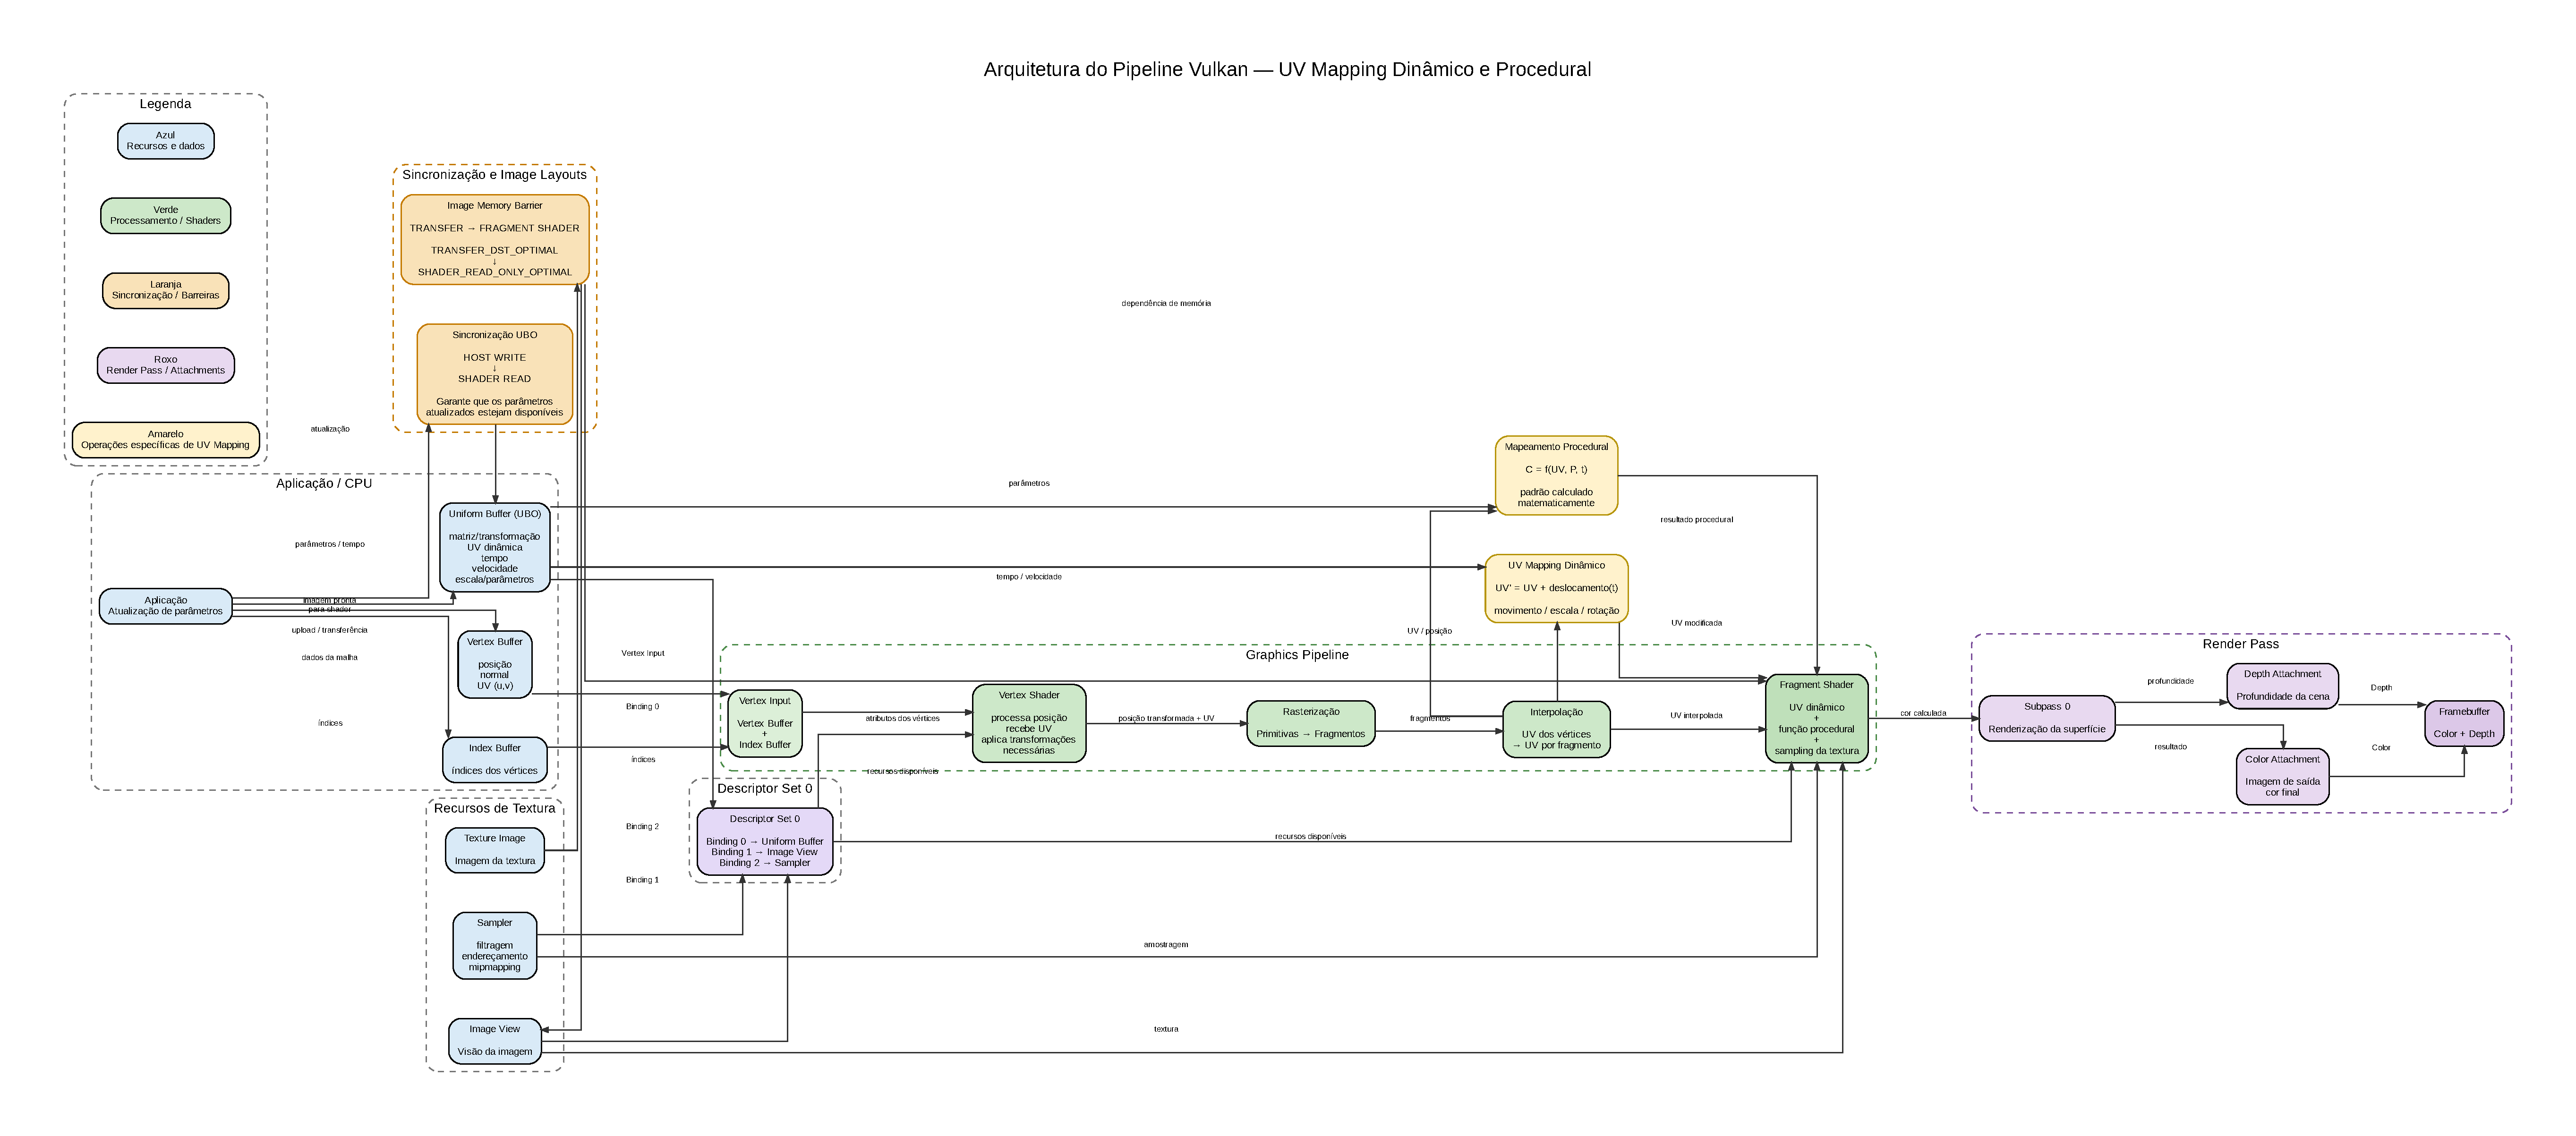
\includegraphics[width=\textwidth,height=0.80\textheight,keepaspectratio]{diagrama/pipeline_vulkan.pdf}
    \caption{Arquitetura do pipeline Vulkan aplicada ao UV mapping dinâmico e procedural, conforme a implementação.}
    \label{fig:pipeline-vulkan}
    \vspace{4pt}
    \small
    \begin{tabular}{@{}l@{\hspace{6pt}}l@{\hspace{14pt}}l@{\hspace{6pt}}l@{}}
    \colorbox[HTML]{D9EAF7}{\strut\hspace{1.2em}} & dados e recursos &
    \colorbox[HTML]{CDE8C9}{\strut\hspace{1.2em}} & estágios e shaders \\
    \colorbox[HTML]{F9E2B8}{\strut\hspace{1.2em}} & sincronização &
    \colorbox[HTML]{E4D9F7}{\strut\hspace{1.2em}} & descriptor set e render pass \\
    \colorbox[HTML]{FFF2CC}{\strut\hspace{1.2em}} & operações de UV mapping &
    \(\longrightarrow\) / \textcolor[HTML]{C47A00}{\(\dashrightarrow\)} & fluxo de dados / sincronização \\
    \end{tabular}
\end{figure}

\section{Recursos usados pela técnica}

\begin{table}[H]
\centering
\caption{Recursos Vulkan da implementação e o papel de cada um no UV mapping.}
\label{tab:recursos-vulkan}
\small
\begin{tabular}{p{2.5cm}p{4.3cm}p{3.5cm}p{3.5cm}}
\toprule
\textbf{Recurso} & \textbf{Configuração} & \textbf{Conteúdo} & \textbf{Atualização} \\
\midrule
Vertex Buffer & \texttt{DEVICE\_LOCAL}, enviado via \textit{staging buffer} & 2.399 vértices de 32 bytes (posição, normal, UV) & Uma vez, na inicialização \\
Index Buffer & \texttt{DEVICE\_LOCAL}, \texttt{UINT32} & 12.636 índices (4.212 triângulos) & Uma vez \\
Uniform Buffer & \texttt{HOST\_VISIBLE | HOST\_COHERENT}, mapeado permanentemente; um por imagem da swapchain & 208 bytes: \(M\), \(V\), \(P\), \texttt{time}, \texttt{mode} & A cada quadro (\texttt{memcpy}) \\
Imagem de textura & \texttt{R8G8B8A8\_SRGB}, \(512\times512\), \texttt{mipLevels = 1} & Cor base do modelo & Uma vez \\
Sampler & \texttt{LINEAR}, \texttt{REPEAT} nos três eixos, anisotropia no máximo do dispositivo & Filtragem e endereçamento & Imutável \\
\bottomrule
\end{tabular}
\end{table}

O Vertex Buffer usa um único binding (0), com \textit{stride} de 32 bytes e taxa por vértice. Cada vértice tem três atributos: posição em \texttt{location 0} (\texttt{R32G32B32\_SFLOAT}, offset 0), normal em \texttt{location 1} (\texttt{R32G32B32\_SFLOAT}, offset 12) e UV em \texttt{location 2} (\texttt{R32G32\_SFLOAT}, offset 24). O Index Buffer é uma lista contínua de inteiros de 32 bits, três por triângulo.

A divisão segue a frequência de atualização de cada dado. Geometria e textura nunca mudam e ficam em memória \texttt{DEVICE\_LOCAL}, a mais rápida para a GPU ler. Os parâmetros que mudam a cada quadro ficam em memória visível pela CPU. O formato \texttt{SRGB} faz a GPU converter a cor para o espaço linear na leitura, de modo que a filtragem e a iluminação operam sobre valores lineares. A textura é formada por três objetos \cite{vulkan}:
\begin{itemize}
    \item a \texttt{VkImage}, que guarda os texels;
    \item a \texttt{VkImageView}, que define como interpretá-los;
    \item o \texttt{VkSampler}, que define como lê-los.
\end{itemize}
Para o UV dinâmico, o sampler é tão importante quanto o shader: o modo \texttt{REPEAT} permite que \(u + 0{,}10\,t\) continue lendo a textura depois de ultrapassar 1, e a filtragem \texttt{LINEAR} evita que o deslocamento lento da textura ``salte'' de um texel para o próximo.

\section{Fluxo de dados entre os estágios}

\begin{table}[H]
\centering
\caption{Estágios do pipeline: o que entra, o que sai e quais recursos são compartilhados.}
\label{tab:estagios}
\small
\begin{tabular}{p{2.5cm}p{3.6cm}p{3.6cm}p{4.1cm}}
\toprule
\textbf{Estágio} & \textbf{Entra} & \textbf{Sai} & \textbf{Recursos usados} \\
\midrule
Aplicação (CPU) & Tempo do relógio, tecla do modo & \(M\), \(V\), \(P\), \texttt{time}, \texttt{mode} & Uniform Buffer da imagem atual \\
Vertex Input & Vertex e Index Buffers & Posição, normal e UV de cada vértice & Vertex Buffer (32 bytes por vértice), Index Buffer \\
Vertex Shader & Atributos do vértice, matrizes & \texttt{gl\_Position}, \texttt{fragUV}, \texttt{fragNormal} & Binding 0 (UBO) \\
Rasterização & Triângulos em espaço de recorte & Fragmentos com UV e normal interpolados (Eq.~\ref{eq:perspectiva}) & Depth attachment (teste de profundidade) \\
Fragment Shader & \texttt{fragUV}, \texttt{fragNormal}, \texttt{time}, \texttt{mode}, textura & Cor final (\texttt{outColor}) & Binding 0 (UBO), binding 1 (textura e sampler) \\
Saída de cor & Cor do fragmento & Pixel no color attachment & Color attachment, framebuffer, swapchain \\
\bottomrule
\end{tabular}
\end{table}

Dois recursos são compartilhados entre estágios: o Uniform Buffer, lido pelos dois shaders, e o depth attachment, escrito e testado durante a rasterização. A textura só é lida pelo fragment shader.

\section{Descriptor Sets e Bindings}

Um \textit{descriptor} é a forma como o Vulkan informa a um shader onde está um recurso. Os descriptors são agrupados em \textit{descriptor sets}, cujo formato é declarado por um \texttt{VkDescriptorSetLayout}. A implementação usa um único set (\texttt{set = 0}) com dois bindings, criados em \texttt{createDescriptorSetLayout}.

\begin{table}[H]
\centering
\caption{Layout do Descriptor Set 0 na implementação.}
\label{tab:descriptor-impl}
\small
\begin{tabular}{cp{4.4cm}p{3.0cm}p{4.6cm}}
\toprule
\textbf{Binding} & \textbf{Tipo} & \textbf{Estágios} & \textbf{Declaração GLSL} \\
\midrule
0 & \texttt{UNIFORM\_BUFFER} & Vertex e Fragment & \texttt{uniform Parameters \{...\} params} \\
1 & \texttt{COMBINED\_IMAGE\_SAMPLER} & Fragment & \texttt{uniform sampler2D baseTexture} \\
\bottomrule
\end{tabular}
\end{table}

O binding~0 é visível nos dois estágios porque o vertex shader usa as matrizes e o fragment shader usa \texttt{time} e \texttt{mode}. O binding~1 é declarado só para o fragment shader, o único que lê a textura. Restringir os \texttt{stageFlags} ao necessário informa ao driver quais estágios precisam enxergar cada recurso. São alocados tantos descriptor sets quantas são as imagens da swapchain, cada um apontando para o seu próprio Uniform Buffer. Assim, a CPU não sobrescreve o \texttt{time} de um quadro enquanto a GPU ainda lê o anterior. O set de cada imagem é ligado uma única vez, com \texttt{vkCmdBindDescriptorSets}, no command buffer daquela imagem.

\subsection{Do projeto à implementação}
\label{sec:projeto-impl}

O projeto inicial da arquitetura (feito antes da implementação, junto com o pseudocódigo em \texttt{pseudocodigo/}) previa três bindings: o Uniform Buffer (0), a imagem (\texttt{SAMPLED\_IMAGE}, 1) e o sampler (\texttt{SAMPLER}, 2), separados. Na implementação, imagem e sampler foram unidos em um \texttt{COMBINED\_IMAGE\_SAMPLER}. As duas formas são válidas, e a escolha depende de quantas texturas existem. Com uma textura e um sampler, o descriptor combinado é mais simples: um binding e uma escrita de descriptor a menos, e o GLSL usa \texttt{sampler2D} diretamente. A separação compensa quando muitas texturas compartilham as mesmas regras de filtragem, por exemplo em um material com cor, normal e rugosidade, em que um único \texttt{VkSampler} é reutilizado.

O Uniform Buffer também mudou. O projeto previa os campos \texttt{uvVelocity} e \texttt{uvScale}. A implementação os trocou por \texttt{time} e \texttt{mode} e deixou as velocidades como constantes no shader, porque elas não variam em tempo de execução. O campo \texttt{mode} seleciona qual dos cinco cálculos o fragment shader executa.

\subsection{Layout de memória do Uniform Buffer (std140)}

O GLSL usa o layout \texttt{std140} para blocos \texttt{uniform}, e a struct C++ precisa ter os mesmos deslocamentos em bytes. A implementação verifica isso em tempo de compilação com \texttt{static\_assert}:

\begin{verbatim}
struct UniformBufferObject {
    glm::mat4 model;       // offset   0
    glm::mat4 view;        // offset  64
    glm::mat4 projection;  // offset 128
    float     time;        // offset 192
    int32_t   mode;        // offset 196
    float     padding[2];  // total: 208 bytes
};
\end{verbatim}

Se um campo fosse reordenado na struct sem a mesma alteração no shader, o tempo seria lido como lixo e a animação pararia, sem nenhum erro de validação. A verificação transforma esse problema em erro de build.

\section{Push constants}

Push constants são uma segunda forma de enviar dados ao shader, sem buffer nem descriptor. Os valores são gravados diretamente no command buffer com \texttt{vkCmdPushConstants} \cite{vkpushconstants} e declarados no shader como \texttt{layout(push\_constant)}. O espaço é pequeno: o limite \texttt{maxPushConstantsSize} tem mínimo garantido de 128 bytes, ou 256 bytes em dispositivos com Vulkan~1.4 \cite{vkmapping,vklimits}. Em troca, a atualização dispensa memória mapeada e um buffer por quadro em execução.

Os dados que mais mudam no UV dinâmico são os candidatos ideais. O par \texttt{time} e \texttt{mode} ocupa 8 bytes; as três matrizes (192 bytes) não cabem no mínimo garantido. Com push constants, o shader e a aplicação ficariam assim:

\begin{verbatim}
layout(push_constant) uniform Animation { float time; int mode; } anim;

vkCmdPushConstants(cmd, pipelineLayout, VK_SHADER_STAGE_FRAGMENT_BIT,
                   0, sizeof(Animation), &anim);
\end{verbatim}

A implementação mantém tudo no Uniform Buffer por uma razão concreta. Os command buffers são gravados uma única vez, em \texttt{createCommandBuffers}, um por imagem da swapchain, e depois apenas reenviados. Como o valor de uma push constant fica gravado dentro do command buffer, usá-las exigiria regravá-lo a cada quadro. Com o Uniform Buffer, os command buffers continuam estáticos e só os 208 bytes do buffer mapeado são reescritos. Para uma versão seguinte, a divisão mais adequada é híbrida: matrizes no Uniform Buffer e \texttt{time}/\texttt{mode} em push constants, com o command buffer regravado por quadro. Essa é a abordagem mais comum em cenas que mudam continuamente, e o custo de gravar um único \textit{draw call} é desprezível.

\section{Render Pass e Subpass}

A implementação usa um Render Pass com um único subpass (Subpass~0), que desenha o modelo, e dois attachments:
\begin{itemize}
    \item \textbf{Color attachment} (formato da swapchain): é limpo no início (\texttt{LOAD\_OP\_CLEAR}), gravado no fim (\texttt{STORE\_OP\_STORE}) e entregue em \texttt{PRESENT\_SRC\_KHR} para ser exibido. Recebe a cor final do fragment shader.
    \item \textbf{Depth attachment} (\texttt{D32\_SFLOAT} ou o melhor formato disponível): é limpo a cada quadro e descartado no fim (\texttt{STORE\_OP\_DONT\_CARE}), porque a profundidade só serve para decidir a visibilidade dentro do próprio quadro.
\end{itemize}
Os dois attachments são ligados a um Framebuffer por imagem da swapchain. Um único subpass basta porque a técnica não precisa de pós-processamento: todo o UV mapping acontece no fragment shader do mesmo passo.

\section{Sincronização: barreiras, layouts e dependências}

\textbf{Transições de layout e barreiras da textura.} A textura passa por duas transições de layout, cada uma com uma \textit{image memory barrier}, criadas em \texttt{transitionImageLayout}:

\begin{table}[H]
\centering
\caption{Barreiras de memória da textura na implementação.}
\label{tab:image-barrier}
\small
\begin{tabular}{p{2.9cm}p{5.2cm}p{5.6cm}}
\toprule
\textbf{Campo} & \textbf{Barreira 1} & \textbf{Barreira 2} \\
\midrule
Recurso & Imagem da textura & Imagem da textura \\
Etapa anterior & \texttt{TOP\_OF\_PIPE} (nenhuma) & \texttt{TRANSFER} \\
Acesso anterior & nenhum & escrita de transferência \\
Etapa posterior & \texttt{TRANSFER} & \texttt{FRAGMENT\_SHADER} \\
Acesso posterior & escrita de transferência & leitura no shader \\
Layout anterior & \texttt{UNDEFINED} & \texttt{TRANSFER\_DST\_OPTIMAL} \\
Layout posterior & \texttt{TRANSFER\_DST\_OPTIMAL} & \texttt{SHADER\_READ\_ONLY\_OPTIMAL} \\
Motivo & Colocar a imagem no layout que aceita a cópia do staging buffer (\texttt{vkCmdCopyBufferToImage}). & Garantir que a cópia terminou e está visível antes da primeira amostragem; sem ela, o shader poderia ler uma textura parcialmente copiada. \\
\bottomrule
\end{tabular}
\end{table}

\textbf{Dependência do subpass e transições dos attachments.} As transições dos attachments são feitas pelo próprio Render Pass, sem barreiras explícitas, e sincronizadas por uma \texttt{VkSubpassDependency} de \texttt{VK\_SUBPASS\_EXTERNAL} para o Subpass~0:

\begin{table}[H]
\centering
\caption{Dependência do subpass e transições dos attachments.}
\label{tab:subpass-dep}
\footnotesize
\begin{tabular}{p{2.4cm}p{5.0cm}p{6.3cm}}
\toprule
\textbf{Campo} & \textbf{Color attachment} & \textbf{Depth attachment} \\
\midrule
Recurso & Imagem da swapchain & Imagem de profundidade \\
Etapa anterior & \texttt{COLOR\_ATTACHMENT\_OUTPUT} (quadro anterior) & \texttt{LATE\_FRAGMENT\_TESTS} (quadro anterior) \\
Acesso anterior & --- & escrita de profundidade \\
Etapa posterior & \texttt{COLOR\_ATTACHMENT\_OUTPUT} & \texttt{EARLY\_FRAGMENT\_TESTS} \\
Acesso posterior & escrita de cor & escrita de profundidade \\
Layout anterior & \texttt{UNDEFINED} & \texttt{UNDEFINED} \\
Layout no subpass & \texttt{COLOR\_ATTACHMENT\_OPTIMAL} & \texttt{DEPTH\_STENCIL\_ATTACHMENT\_OPTIMAL} \\
Layout final & \texttt{PRESENT\_SRC\_KHR} & \texttt{DEPTH\_STENCIL\_ATTACHMENT\_OPTIMAL} \\
Motivo & Não escrever na imagem antes de ela ser liberada pela apresentação anterior & Não limpar a profundidade enquanto o quadro anterior ainda a testa e grava \\
\bottomrule
\end{tabular}
\end{table}

O layout anterior \texttt{UNDEFINED} indica que o conteúdo antigo pode ser descartado, o que é correto porque os dois attachments são limpos no início do passo.

\textbf{Dependências entre CPU e GPU.} A cada quadro, a aplicação:
\begin{enumerate}
    \item espera a fence do quadro em execução (\texttt{MAX\_FRAMES\_IN\_FLIGHT = 2});
    \item adquire a próxima imagem da swapchain, com um semáforo (\texttt{imageAvailable}) que fará a GPU esperar a imagem ficar livre;
    \item espera a fence associada àquela imagem (\texttt{imagesInFlight}). Como o Uniform Buffer é um por imagem, é essa espera que garante que a GPU terminou de ler o buffer que será reescrito;
    \item mede o tempo e copia \(M\), \(V\), \(P\), \texttt{time} e \texttt{mode} para o Uniform Buffer daquela imagem (\texttt{updateUniformBuffer});
    \item submete o command buffer, que sinaliza o semáforo \texttt{renderFinished}, esperado pela apresentação.
\end{enumerate}
A escrita da CPU fica visível para a GPU sem barreira explícita porque a memória é \texttt{HOST\_COHERENT} e a submissão à fila garante a ordem entre a escrita no host e as leituras dos shaders.

\section{Onde cada cálculo é feito}
\label{sec:onde-calculo}

Em Vulkan, a aplicação escolhe se um cálculo roda na CPU (uma vez por quadro), no vertex shader (por vértice) ou no fragment shader (por pixel). Com 2.399 vértices contra até 480.000 pixels (Capítulo~\ref{chap:equacoes}), essa é a decisão de desempenho mais importante da técnica.
\begin{itemize}
    \item \textbf{CPU:} medir o tempo, montar \(M\), \(V\), \(P\) e, se houvesse rotação de UV, calcular \(\cos\theta\) e \(\sin\theta\).
    \item \textbf{Vertex shader:} transformações lineares do UV (translação, escala, rotação), que interpoladas dão o mesmo resultado que se fossem feitas por fragmento.
    \item \textbf{Fragment shader:} tudo o que é não linear (ondulação, padrão procedural, grade) e a amostragem da textura.
\end{itemize}
O projeto fazia a translação no vertex shader. A implementação a moveu para o fragment shader, dentro de \texttt{dynamicUV}, junto com a ondulação. Isso mantém todo o efeito em uma função legível, ao custo de uma soma por pixel em vez de uma por vértice, diferença desprezível neste caso.

\section{Otimizações: aplicadas e pendentes}

\begin{table}[H]
\centering
\caption{Otimizações relevantes para a técnica e sua situação na implementação.}
\label{tab:otimizacoes}
\small
\begin{tabular}{p{3.6cm}p{1.6cm}p{8.6cm}}
\toprule
\textbf{Otimização} & \textbf{Situação} & \textbf{Efeito} \\
\midrule
Geometria em \texttt{DEVICE\_LOCAL} via staging & Aplicada & A GPU lê vértices e índices da memória mais rápida; a cópia é feita uma vez com \texttt{vkCmdCopyBuffer}. \\
Uniform Buffer mapeado permanentemente & Aplicada & Sem \texttt{vkMapMemory}/\texttt{vkUnmapMemory} por quadro: a atualização é um \texttt{memcpy} de 208 bytes. \\
Um Uniform Buffer por imagem e 2 quadros em execução & Aplicada & A CPU prepara o próximo quadro enquanto a GPU desenha o atual, sem escrever em um buffer em uso. \\
Filtragem anisotrópica & Aplicada & Reduz o borrão em superfícies inclinadas; ativada só se o dispositivo suportar. \\
Command buffers pré-gravados & Aplicada & Nenhum custo de gravação por quadro; é o motivo de \texttt{time} estar no Uniform Buffer. \\
\addlinespace
Mipmaps & \textbf{Pendente} & A textura tem \texttt{mipLevels = 1}, o que causa aliasing com o modelo pequeno na tela. A correção é criar \(\lfloor\log_2 512\rfloor+1=10\) níveis e gerá-los com \texttt{vkCmdBlitImage} \cite{vkmipmaps}, ao custo de \(1/3\) a mais de memória \cite[p.~9]{heckbert1986}. \\
Specialization constants por modo & Pendente & O shader escolhe o modo com \texttt{if} sobre \texttt{params.mode}. Não há divergência entre threads, pois o valor é igual para todos os fragmentos, mas o shader contém os cinco caminhos. Com \texttt{VkSpecializationInfo}, cada modo viraria um pipeline só com o código necessário. \\
Transformações lineares no vertex shader & Pendente & A translação de \texttt{dynamicUV} poderia rodar de 2.399 a 12.636 vezes por quadro, em vez de até 480.000. \\
Índices de 16 bits & Pendente & O glTF guarda os índices em 16 bits, e a implementação os converte para 32. Com menos de 65.536 vértices, \texttt{UINT16} reduziria o Index Buffer à metade. \\
Tempo periódico na CPU & Pendente & Enviar \(t \bmod T\) em vez de \(t\) evita a perda de precisão do \texttt{float} após muitas horas (Capítulo~\ref{chap:fundamentacao}). \\
\bottomrule
\end{tabular}
\end{table}

\section{Justificativa das decisões arquiteturais}

\begin{itemize}
    \item \textbf{Um único subpass:} todo o efeito acontece no fragment shader do mesmo passo. Não há pós-processamento que justifique um segundo subpass ou render pass.
    \item \textbf{Geometria e textura em memória \texttt{DEVICE\_LOCAL}:} são enviadas uma vez e lidas em todos os quadros, então pagam o custo do staging uma única vez.
    \item \textbf{Parâmetros em um Uniform Buffer por imagem da swapchain:} mantêm os command buffers estáticos e evitam escrever em um buffer que a GPU ainda está lendo.
    \item \textbf{Sampler em \texttt{REPEAT} com filtragem linear:} é o que torna possível deslocar o UV indefinidamente sem costura nem saltos de texel.
    \item \textbf{Cálculo do efeito no fragment shader:} a ondulação e o padrão procedural são não lineares e precisam ser avaliados por pixel. A translação, que é linear, foi mantida junto delas por legibilidade.
    \item \textbf{Descriptor combinado:} com uma única textura, é a organização mais simples e não perde nada em relação a imagem e sampler separados.
\end{itemize}


\chapter{Shaders: pseudocódigo e implementação}
\label{chap:shaders}

\section{Objetivo de cada shader e fluxo entre eles}

A técnica usa dois shaders. Eles começaram como pseudocódigo em sintaxe GLSL (arquivos originais em \texttt{pseudocodigo/}) e evoluíram para os shaders compiláveis da implementação (\texttt{código/shaders/uv\_mapping.vert} e \texttt{uv\_mapping.frag}), que são apresentados aqui como a versão final.

\begin{itemize}
    \item \textbf{Vertex shader} (\texttt{uv\_mapping.vert}): transforma a posição de cada vértice para o espaço de recorte e repassa o UV e a normal. Não altera o UV.
    \item \textbf{Fragment shader} (\texttt{uv\_mapping.frag}): recebe o UV já interpolado e, conforme o modo, lê a textura com o UV original ou deslocado, calcula o padrão procedural, mistura os dois ou desenha a grade de depuração. No fim, aplica a iluminação.
\end{itemize}

O fluxo é: atributos do vértice \(\rightarrow\) vertex shader \(\rightarrow\) rasterização, que interpola \texttt{fragUV} e \texttt{fragNormal} com correção de perspectiva (Equação~\eqref{eq:perspectiva}) \(\rightarrow\) fragment shader \(\rightarrow\) cor no color attachment. Os dois shaders compartilham o mesmo bloco \texttt{uniform} (binding~0).

\section{Entradas, saídas e recursos}

\begin{table}[H]
\centering
\caption{Entradas, saídas e recursos dos shaders.}
\label{tab:shader-io}
\small
\begin{tabular}{p{3.0cm}p{2.0cm}p{2.4cm}p{6.4cm}}
\toprule
\textbf{Nome} & \textbf{Tipo} & \textbf{Origem} & \textbf{Significado} \\
\midrule
\texttt{inPosition} & \texttt{vec3} & location 0 & Posição do vértice no espaço do modelo \\
\texttt{inNormal} & \texttt{vec3} & location 1 & Normal do vértice \\
\texttt{inUV} & \texttt{vec2} & location 2 & Coordenada de textura do glTF (\texttt{TEXCOORD\_0}) \\
\texttt{params.model}, \texttt{view}, \texttt{projection} & \texttt{mat4} & binding 0 & Matrizes de modelo (rotação), câmera e projeção \\
\texttt{params.time} & \texttt{float} & binding 0 & Segundos desde o início, \(t\) nas equações \\
\texttt{params.mode} & \texttt{int} & binding 0 & Modo de renderização, de 1 a 5 \\
\texttt{baseTexture} & \texttt{sampler2D} & binding 1 & Textura do modelo com o sampler (\texttt{LINEAR}, \texttt{REPEAT}) \\
\texttt{fragUV}, \texttt{fragNormal} & \texttt{vec2}, \texttt{vec3} & vertex \(\rightarrow\) fragment & UV e normal, interpolados por fragmento \\
\texttt{gl\_Position} & \texttt{vec4} & saída do vertex & Posição em espaço de recorte \\
\texttt{outColor} & \texttt{vec4} & saída do fragment & Cor final do pixel (location 0) \\
\bottomrule
\end{tabular}
\end{table}

\section{Vertex shader}

\begin{small}
\begin{verbatim}
#version 450
layout(set = 0, binding = 0) uniform Parameters {
    mat4 model; mat4 view; mat4 projection;  // matrizes (Eq. 3.2)
    float time; int mode;                    // tempo e modo (1 a 5)
} params;

layout(location = 0) in vec3 inPosition;     // atributos do glTF
layout(location = 1) in vec3 inNormal;
layout(location = 2) in vec2 inUV;
layout(location = 0) out vec2 fragUV;        // vao para o rasterizador
layout(location = 1) out vec3 fragNormal;

void main() {
    // posicao em espaco de recorte: P * V * M * p
    gl_Position = params.projection * params.view * params.model
                * vec4(inPosition, 1.0);
    // o UV do arquivo e repassado sem alteracao; o rasterizador
    // o interpola com correcao de perspectiva
    fragUV = inUV;
    // a matriz model e so rotacao, entao serve tambem para normais
    fragNormal = mat3(params.model) * inNormal;
}
\end{verbatim}
\end{small}

\section{Fragment shader}

\begin{small}
\begin{verbatim}
#version 450
layout(set = 0, binding = 0) uniform Parameters {
    mat4 model; mat4 view; mat4 projection; float time; int mode;
} params;
layout(set = 0, binding = 1) uniform sampler2D baseTexture;
layout(location = 0) in vec2 fragUV;
layout(location = 1) in vec3 fragNormal;
layout(location = 0) out vec4 outColor;

const int MODE_TEXTURE = 1, MODE_DYNAMIC_UV = 2, MODE_PROCEDURAL = 3,
          MODE_BLEND = 4,   MODE_UV_GRID = 5;

// UV DINAMICO (Eqs. 3.5 e 3.6): a malha fica parada, o UV se move
vec2 dynamicUV(vec2 uv, float t) {
    uv.x += t * 0.10;                              // translacao
    uv.x += sin(uv.y * 12.0 + t * 2.0) * 0.015;    // ondulacao em u
    uv.y += cos(uv.x * 12.0 + t * 1.5) * 0.015;    // ondulacao em v
    return uv;   // pode sair de [0,1]: o sampler REPEAT da a volta
}

// PADRAO PROCEDURAL (Eq. 3.11): cor gerada por funcoes, sem imagem.
// Retorna a cor em rgb e a "energia" da onda em a.
vec4 proceduralPattern(vec2 uv, float t) {
    uv.x += t * 0.40;                              // deslocamento
    uv.y += sin(t * 1.2) * 0.10;
    float dx = sin(uv.y * 14.0 + t * 2.0) * 0.08;  // distorcao: as duas
    float dy = cos(uv.x * 12.0 - t * 1.5) * 0.08;  // partes usam o uv
    uv += vec2(dx, dy);                            // anterior a ela
    float w1 = sin(uv.x * 20.0 + uv.y * 8.0 + t * 4.0);   // 3 ondas
    float w2 = sin(uv.y * 24.0 - uv.x * 6.0 - t * 3.0);
    float w3 = sin((uv.x + uv.y) * 18.0 + t * 2.0);
    float e = ((w1 + w2 + w3) / 3.0) * 0.5 + 0.5;  // normaliza p/ [0,1]
    vec2 g = fract(uv * 8.0);                      // grade 8x8 (Eq. 3.8)
    float grid = max(smoothstep(0.46, 0.50, abs(g.x - 0.5)),
                     smoothstep(0.46, 0.50, abs(g.y - 0.5)));
    vec3 c = mix(vec3(0.005, 0.015, 0.12), vec3(0.0, 0.18, 0.85), e);
    c = mix(c, vec3(0.0, 0.85, 1.0), smoothstep(0.55, 0.90, e));
    c = mix(c, vec3(0.65, 1.0, 1.0), smoothstep(0.90, 1.0, e));
    c = mix(c, c * 0.35, grid * 0.25);             // escurece a grade
    c += vec3(0.0, 0.25, 0.35) * pow(e, 3.0);      // brilho
    return vec4(c, e);
}

// GRADE UV (depuracao): U em vermelho, V em verde, xadrez 10x10
vec3 uvGrid(vec2 uv) {
    vec2 cells = uv * 10.0;
    float checker = mod(floor(cells.x) + floor(cells.y), 2.0);
    vec2 d = abs(fract(cells) - 0.5);
    float line = smoothstep(0.44, 0.48, max(d.x, d.y));
    vec3 c = vec3(fract(uv.x), fract(uv.y), 0.2) * (0.65 + 0.35 * checker);
    return mix(c, vec3(1.0), line);
}

void main() {
    float t = params.time;
    // iluminacao difusa (Eq. 3.14); a normal interpolada e renormalizada
    vec3 n = normalize(fragNormal);
    float diffuse = max(dot(n, normalize(vec3(0.4, 0.8, 0.6))), 0.0);
    float lighting = 0.35 + 0.65 * diffuse;
    vec3 color;
    if (params.mode == MODE_TEXTURE)
        color = texture(baseTexture, fragUV).rgb * lighting;
    else if (params.mode == MODE_DYNAMIC_UV)
        color = texture(baseTexture, dynamicUV(fragUV, t)).rgb * lighting;
    else if (params.mode == MODE_PROCEDURAL)
        color = proceduralPattern(fragUV, t).rgb * (0.55 + 0.45 * diffuse);
    else if (params.mode == MODE_UV_GRID)
        color = uvGrid(fragUV) * lighting;
    else {  // MODE_BLEND (e qualquer valor fora de 1..5)
        vec3 tex = texture(baseTexture, dynamicUV(fragUV, t)).rgb * lighting;
        vec4 p = proceduralPattern(fragUV, t);
        color = mix(tex, p.rgb, smoothstep(0.45, 0.95, p.a) * 0.75);
    }
    outColor = vec4(color, 1.0);
}
\end{verbatim}
\end{small}

\section{Equações e variáveis}

Cada cálculo do shader corresponde a uma equação do Capítulo~\ref{chap:equacoes}, onde estão o significado de cada variável e o estágio em que ela é executada: posição (Eq.~\ref{eq:mvp}), translação (Eq.~\ref{eq:translacao}), ondulação (Eq.~\ref{eq:onda}), repetição (Eq.~\ref{eq:repeat}), escala (Eq.~\ref{eq:escala}), padrão procedural e misturas (Eqs.~\ref{eq:procedural} e~\ref{eq:mix}) e iluminação (Eq.~\ref{eq:lambert}). As funções GLSL usadas são \texttt{mix(a,b,x)} \(= a(1-x)+bx\); \texttt{smoothstep(e0,e1,x)}, uma transição suave de 0 a 1 entre \(e_0\) e \(e_1\); \texttt{fract(x)} \(= x-\lfloor x\rfloor\); e \texttt{normalize}, que divide o vetor pela sua norma.

\section{Condições e laços}

O fragment shader tem uma única cadeia de condições, sobre \texttt{params.mode}, que escolhe um de cinco cálculos. Como \texttt{mode} vem do Uniform Buffer, o valor é o mesmo para todos os fragmentos do quadro: todas as threads seguem o mesmo ramo e não há divergência. Não há laços: as três ondas do padrão procedural são uma soma de tamanho fixo, escrita explicitamente, e nenhum cálculo depende de vizinhos ou de iterações. O critério de parada, portanto, não se aplica. Cada fragmento executa um número constante de operações (Tabela~\ref{tab:custo-modos}).

\section{Amostragem da textura}

A textura é lida com \texttt{texture(baseTexture, uv)} nos modos 1, 2 e 4. O sampler é configurado na aplicação (Capítulo~\ref{chap:vulkan}) com:
\begin{itemize}
    \item filtragem \texttt{LINEAR} na ampliação e na redução, que interpola os quatro texels mais próximos;
    \item endereçamento \texttt{REPEAT}, que aplica a Equação~\eqref{eq:repeat} ao UV deslocado;
    \item anisotropia no máximo suportado pela GPU;
    \item modo de mipmap \texttt{LINEAR}.
\end{itemize}
Como a imagem tem um único nível, o nível de detalhe calculado pela GPU (Equação~\eqref{eq:lod}) não tem efeito. Essa limitação está registrada na Tabela~\ref{tab:otimizacoes}. O padrão procedural e a grade não leem textura: são calculados diretamente a partir do UV.

\section{Tratamento de limites e valores inválidos}

\begin{itemize}
    \item \textbf{UV fora de \([0,1]\):} o deslocamento faz \(u\) crescer sem limite. Quem trata isso é o sampler (\texttt{REPEAT}), e não o shader. A grade usa \texttt{fract} pelo mesmo motivo.
    \item \textbf{Normal interpolada:} não é unitária, por isso é renormalizada. Uma normal nula produziria NaN, mas o modelo glTF sempre fornece normais.
    \item \textbf{Luz por trás da superfície:} \texttt{max(dot, 0)} impede iluminação negativa, e o termo constante de 0,35 evita regiões totalmente pretas.
    \item \textbf{Energia procedural:} a soma das ondas, no intervalo \([-3,3]\), é normalizada para \([0,1]\) antes de servir de peso nas misturas, o que garante que \texttt{mix} e \texttt{smoothstep} recebam valores válidos.
    \item \textbf{Cor acima de 1:} o brilho do padrão procedural pode somar até \(0{,}35\) ao canal azul e levar a cor acima de 1. O shader não aplica \texttt{clamp}: como o color attachment usa um formato normalizado de 8 bits, a GPU limita cada canal a \([0,1]\) na escrita.
    \item \textbf{Modo inválido:} qualquer valor fora de 1 a 5 cai no último ramo (mistura). Na aplicação, o valor só muda pelas teclas 1 a 5.
\end{itemize}

\section{Resultado esperado e relação com a técnica}

O vertex shader produz a posição do vértice na tela, e o fragment shader produz a cor de cada pixel do modelo. A Figura~\ref{fig:app-modos} mostra os modos 1, 3, 4 e 5; o modo~2 está na Figura~\ref{fig:app-uv-dinamico}.

\begin{figure}[H]
    \centering
    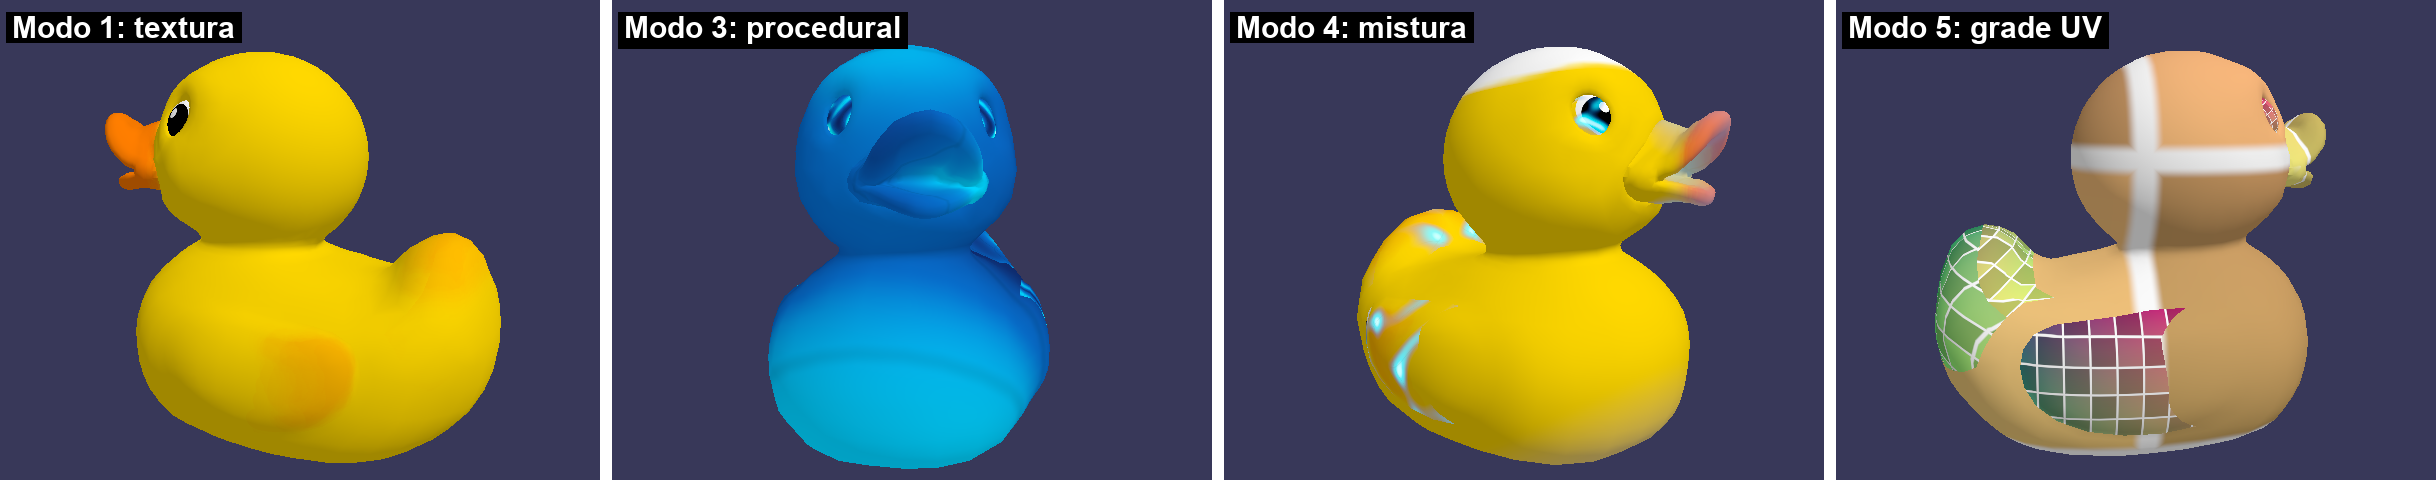
\includegraphics[width=\textwidth]{imagens/marcadas/app_modos.png}
    \caption{Resultado dos shaders na implementação (capturas próprias, \texttt{código/evidencias/}).}
    \label{fig:app-modos}
\end{figure}

Resultado esperado de cada modo:
\begin{enumerate}
    \item a textura original do modelo;
    \item a mesma textura deslizando e ondulando sobre a malha parada (Figura~\ref{fig:app-uv-dinamico});
    \item ondas azuis e ciano geradas sem imagem;
    \item a textura deslizando com ondas de luz por cima;
    \item a grade de depuração, que revela o esticamento e as costuras do UV.
\end{enumerate}
O modo~2 implementa o UV mapping dinâmico (a parametrização muda a cada quadro), o modo~3 o mapeamento procedural (a cor vem de uma função) e o modo~4 a combinação dos dois.


\chapter{Aplicações práticas}
\label{chap:aplicacoes}

Este capítulo apresenta produtos comerciais e ferramentas em uso na indústria que implementam UV mapping dinâmico ou mapeamento procedural, indicando para cada um o recurso específico, a equação correspondente no Capítulo~\ref{chap:equacoes} e a fonte que comprova o uso.

\section{Motores de jogo: UV dinâmico como recurso de material}

\subsection{Unreal Engine: nó \textit{Panner}}

No editor de materiais da Unreal Engine, o nó \textit{Panner} gera coordenadas UV que mudam de acordo com a entrada de tempo \cite{unrealpanner}. Ele recebe as coordenadas originais e uma entrada de tempo, e tem duas propriedades de velocidade, \textit{Speed X} e \textit{Speed Y}, uma para cada direção. É exatamente a Equação~\eqref{eq:translacao} (\(u'=u+s_u t\), \(v'=v+s_v t\)), empacotada como um bloco visual para artistas. A documentação oficial apresenta o nó como a forma de criar texturas ``em deslocamento, ou em movimento'' \cite{unrealpanner}. O Rocket League é desenvolvido sobre a Unreal Engine~3 \cite{substance}.

\subsection{Unity: nó \textit{Tiling And Offset} do Shader Graph}

No Shader Graph da Unity, o nó \textit{Tiling And Offset} aplica à coordenada de entrada a operação \texttt{Out = UV * Tiling + Offset} \cite{unitytiling}, que combina a escala (Equação~\eqref{eq:escala}) e a translação (Equação~\eqref{eq:translacao}). Segundo a documentação, o nó é ``comumente usado para mapas de detalhe e para rolar texturas ao longo do tempo'' \cite{unitytiling}: basta ligar a saída de um nó de tempo à entrada \textit{Offset}.

\section{Ferramentas de autoria de texturas procedurais}

\subsection{Adobe Substance 3D Designer}

O Substance Designer é um editor de texturas procedurais baseado em grafos de nós. Smelik et al.\ o citam entre os editores visuais por nós de uso disseminado em sistemas comerciais \cite[p.~14]{smelik2014}. O uso em produção está documentado em uma entrevista com Eric Majka, um dos artistas líderes da Psyonix: todos os mapas recentes do Rocket League foram texturizados inteiramente no Designer, com \textit{trim textures} (texturas em faixas reaproveitadas por várias peças) divididas em quartos para facilitar o UV mapping feito pelos modeladores. Os padrões da banda de rodagem dos pneus e os mapas de altura dos aros também são gerados nele \cite{substance}. A ferramenta é procedural na autoria: o artista edita parâmetros e o grafo gera as imagens finais, que o jogo usa como texturas comuns.

\subsection{Blender: nós \textit{Mapping}, \textit{Noise Texture} e \textit{Voronoi Texture}}

O Blender, software livre de modelagem e renderização, oferece os dois lados da técnica como nós de material. O nó \textit{Mapping} ``transforma o vetor de entrada aplicando translação, rotação e escala'' \cite{blendermapping}, a mesma transformação combinada da Equação~\eqref{eq:combinada}. Com um valor animado na translação, ele produz UV dinâmico. Os nós \textit{Noise Texture} e \textit{Voronoi Texture} avaliam, respectivamente, um ruído de Perlin fractal e um ruído de Worley ``nas coordenadas de textura de entrada'' \cite{blendernoise,blendervoronoi}. Na classificação de Dong et al., o primeiro é um ruído de gradiente em grade (método não estruturado, domínio espacial) e o segundo uma textura celular (método estruturado) \cite[pp.~10, 16]{dong2020}.

\section{Modelagem procedural de mundos virtuais}

Smelik et al.\ dedicam uma seção do levantamento aos sistemas disponíveis comercialmente, para mostrar ``como os resultados de pesquisa já estão sendo aplicados na indústria'' \cite[p.~10]{smelik2014}. Os três seguintes estão entre os citados.

\subsection{SpeedTree}

O SpeedTree é um \textit{middleware} para modelagem e renderização de grandes quantidades de vegetação procedural, com ``ampla aplicação nas indústrias de jogos e de cinema'' \cite[p.~11]{smelik2014}. O fabricante o descreve como o conjunto de ferramentas de vegetação padrão da indústria, que combina geradores procedurais com edição manual \cite{speedtree}. Segundo Smelik et al., o próprio motor do SpeedTree anima a vegetação e gerencia o nível de detalhe na renderização \cite[p.~11]{smelik2014}.

\subsection{Esri ArcGIS CityEngine}

O CityEngine é um gerador de cidades baseado em gramáticas CGA \cite[p.~12]{smelik2014}. Na documentação oficial, a modelagem é ``descrita de forma abstrata, em um arquivo de regras'', que refina iterativamente as formas até gerar os edifícios \cite{cityengine}. O produto faz parte da plataforma ArcGIS, de geoprocessamento, e é voltado à geração de cidades e quarteirões inteiros em 3D. Uma regra CGA típica divide a fachada em andares e janelas que se repetem, o que, na textura, corresponde ao ladrilhamento por escala de UV da Equação~\eqref{eq:escala}.

\subsection{SideFX Houdini}

O Houdini permite que designers criem geradores procedurais a partir de pequenos blocos de construção \cite[p.~12]{smelik2014}. Os autores ressaltam, porém, que o uso eficaz exige conhecimento avançado de como projetar esses procedimentos, um exemplo concreto da limitação de controle discutida no Capítulo~\ref{chap:fundamentacao}.

\section{Resumo}

\begin{table}[H]
\centering
\caption{Produtos analisados e sua relação com a técnica.}
\label{tab:aplicacoes}
\small
\begin{tabular}{p{3.0cm}p{3.6cm}p{4.0cm}p{3.4cm}}
\toprule
\textbf{Produto} & \textbf{Recurso} & \textbf{Técnica} & \textbf{Fonte} \\
\midrule
Unreal Engine & Nó \textit{Panner} & UV dinâmico, Eq.~\eqref{eq:translacao} & \cite{unrealpanner} \\
Unity & Nó \textit{Tiling And Offset} & UV dinâmico, Eqs.~\eqref{eq:translacao}~e~\eqref{eq:escala} & \cite{unitytiling} \\
Substance 3D Designer & Grafo de textura procedural & Procedural na autoria (Rocket League) & \cite{substance}, \cite[p.~14]{smelik2014} \\
Blender & \textit{Mapping}, \textit{Noise}, \textit{Voronoi} & UV dinâmico e procedural, Eq.~\eqref{eq:combinada} & \cite{blendermapping,blendernoise,blendervoronoi} \\
SpeedTree & Vegetação procedural & Modelagem procedural e LOD & \cite{speedtree}, \cite[p.~11]{smelik2014} \\
CityEngine & Regras CGA & Modelagem procedural, fachadas por repetição & \cite{cityengine}, \cite[p.~12]{smelik2014} \\
Houdini & Geradores por nós & Modelagem procedural & \cite[p.~12]{smelik2014} \\
\bottomrule
\end{tabular}
\end{table}

Os produtos se dividem em dois grupos. Nos motores de jogo (Unreal, Unity), a técnica é executada em tempo real, a cada quadro, no shader. Nas ferramentas de autoria (Substance, SpeedTree, CityEngine, Houdini), o procedural é usado durante a produção e o resultado é gravado como texturas e malhas comuns. Essa divisão segue o argumento de custo do Capítulo~\ref{chap:fundamentacao}: o que é barato o suficiente roda no shader, e o que é caro ou difícil de controlar é gerado antes.


\chapter{Análise em jogos}
\label{chap:jogos}

Os dois jogos foram jogados pelo grupo em um PlayStation~5. As capturas foram extraídas das transmissões ao vivo feitas por um integrante do grupo no canal \textit{Nerd Geek TV}. Para cada jogo, a ficha traz os itens pedidos na análise: plataforma, situação de gameplay, momento, elemento visual, efeito, benefício e fonte técnica. Depois vêm as capturas marcadas e o vídeo.

Uma ressalva vale para os dois casos. Um jogo comercial não expõe seus shaders, e uma captura mostra só o resultado final. Quando o texto afirma como algo foi produzido, a afirmação vem de uma fonte do estúdio. Quando descreve um efeito observado na tela, ele é apresentado como \textit{compatível} com a técnica, e não como prova da implementação.

\textbf{Como ler as capturas.} Os retângulos amarelos numerados marcam onde o UV mapping está sendo aplicado. A legenda de cada figura explica cada número: qual técnica aparece e em qual equação do Capítulo~\ref{chap:equacoes} ela se encaixa.

\section{Rocket League}

\begin{table}[H]
\centering
\caption{Análise do Rocket League.}
\label{tab:ficha-rl}
\small
\begin{tabular}{p{3.0cm}p{11.0cm}}
\toprule
Jogo & \textit{Rocket League} (Psyonix), motor Unreal Engine~3 \cite{substance} \\
Plataforma & PlayStation~5, executando a versão de PS4 por retrocompatibilidade \cite{rlstore}, em 4K (\textit{checkerboard}) a 60 quadros por segundo com HDR \cite{rlps5} \\
Situação analisada & (a) Partida online e o \textit{replay} automático exibido após um gol; (b) tela inicial, com o carro do jogador em destaque \\
Momento & (a) Logo após o gol que deixou o placar em 4 a 3, faltando 3:18; (b) antes de entrar na partida \\
Elementos visuais & Carroceria, rodas e antena dos carros; bola; piso, faixas e painéis do estádio; rastro do \textit{boost} \\
Efeito produzido & Pinturas e decalques que seguem a forma de cada carro; piso e faixas repetidos em todo o campo; rastro animado atrás do carro ao acelerar \\
Benefício & O mesmo layout UV de cada carro recebe dezenas de pinturas, decalques e rodas, a base da personalização do jogo, sem novos modelos. As \textit{trim textures} reaproveitadas texturizam arenas inteiras com poucas imagens. O rastro animado dá retorno visual da aceleração sem geometria extra \\
Fonte técnica & Entrevista de um dos artistas líderes da Psyonix sobre o uso do Substance Designer no jogo \cite{substance} \\
\bottomrule
\end{tabular}
\end{table}

Segundo a entrevista \cite{substance}:
\begin{itemize}
    \item os mapas recentes foram texturizados inteiramente no Substance Designer, com \textit{trim textures} divididas em quartos para facilitar o UV mapping feito pelos modeladores;
    \item a banda de rodagem dos pneus e o relevo dos aros são gerados proceduralmente no Designer;
    \item um grafo combina mapas de curvatura e espessura com um mapa gerado a partir do layout UV de cada carro para criar os efeitos de borda dos decalques, e é reaplicado a cada carro novo;
    \item máscaras permitem aplicar a cor de cada time.
\end{itemize}
O rastro do \textit{boost} é o efeito em que se espera UV dinâmico: uma faixa animada que acompanha o carro. Em motores como a Unreal, esse tipo de efeito é montado com texturas em deslocamento, como as do nó \textit{Panner} \cite{unrealpanner}. Como o estúdio não detalha a implementação do rastro, e parte dele é feita de partículas (estrelas e fumaça, no item usado pelo jogador na live), ele é tratado aqui apenas como efeito compatível com a técnica.

\textbf{Cena da Figura~\ref{fig:rl-replay}.} Logo após um gol em partida online, o jogo exibe o \textit{replay} da jogada. A câmera acompanha a bola perto do gol, com o carro adversário (azul) e o do jogador (vermelho, marcado ``Você'') no fundo.

\begin{figure}[H]
    \centering
    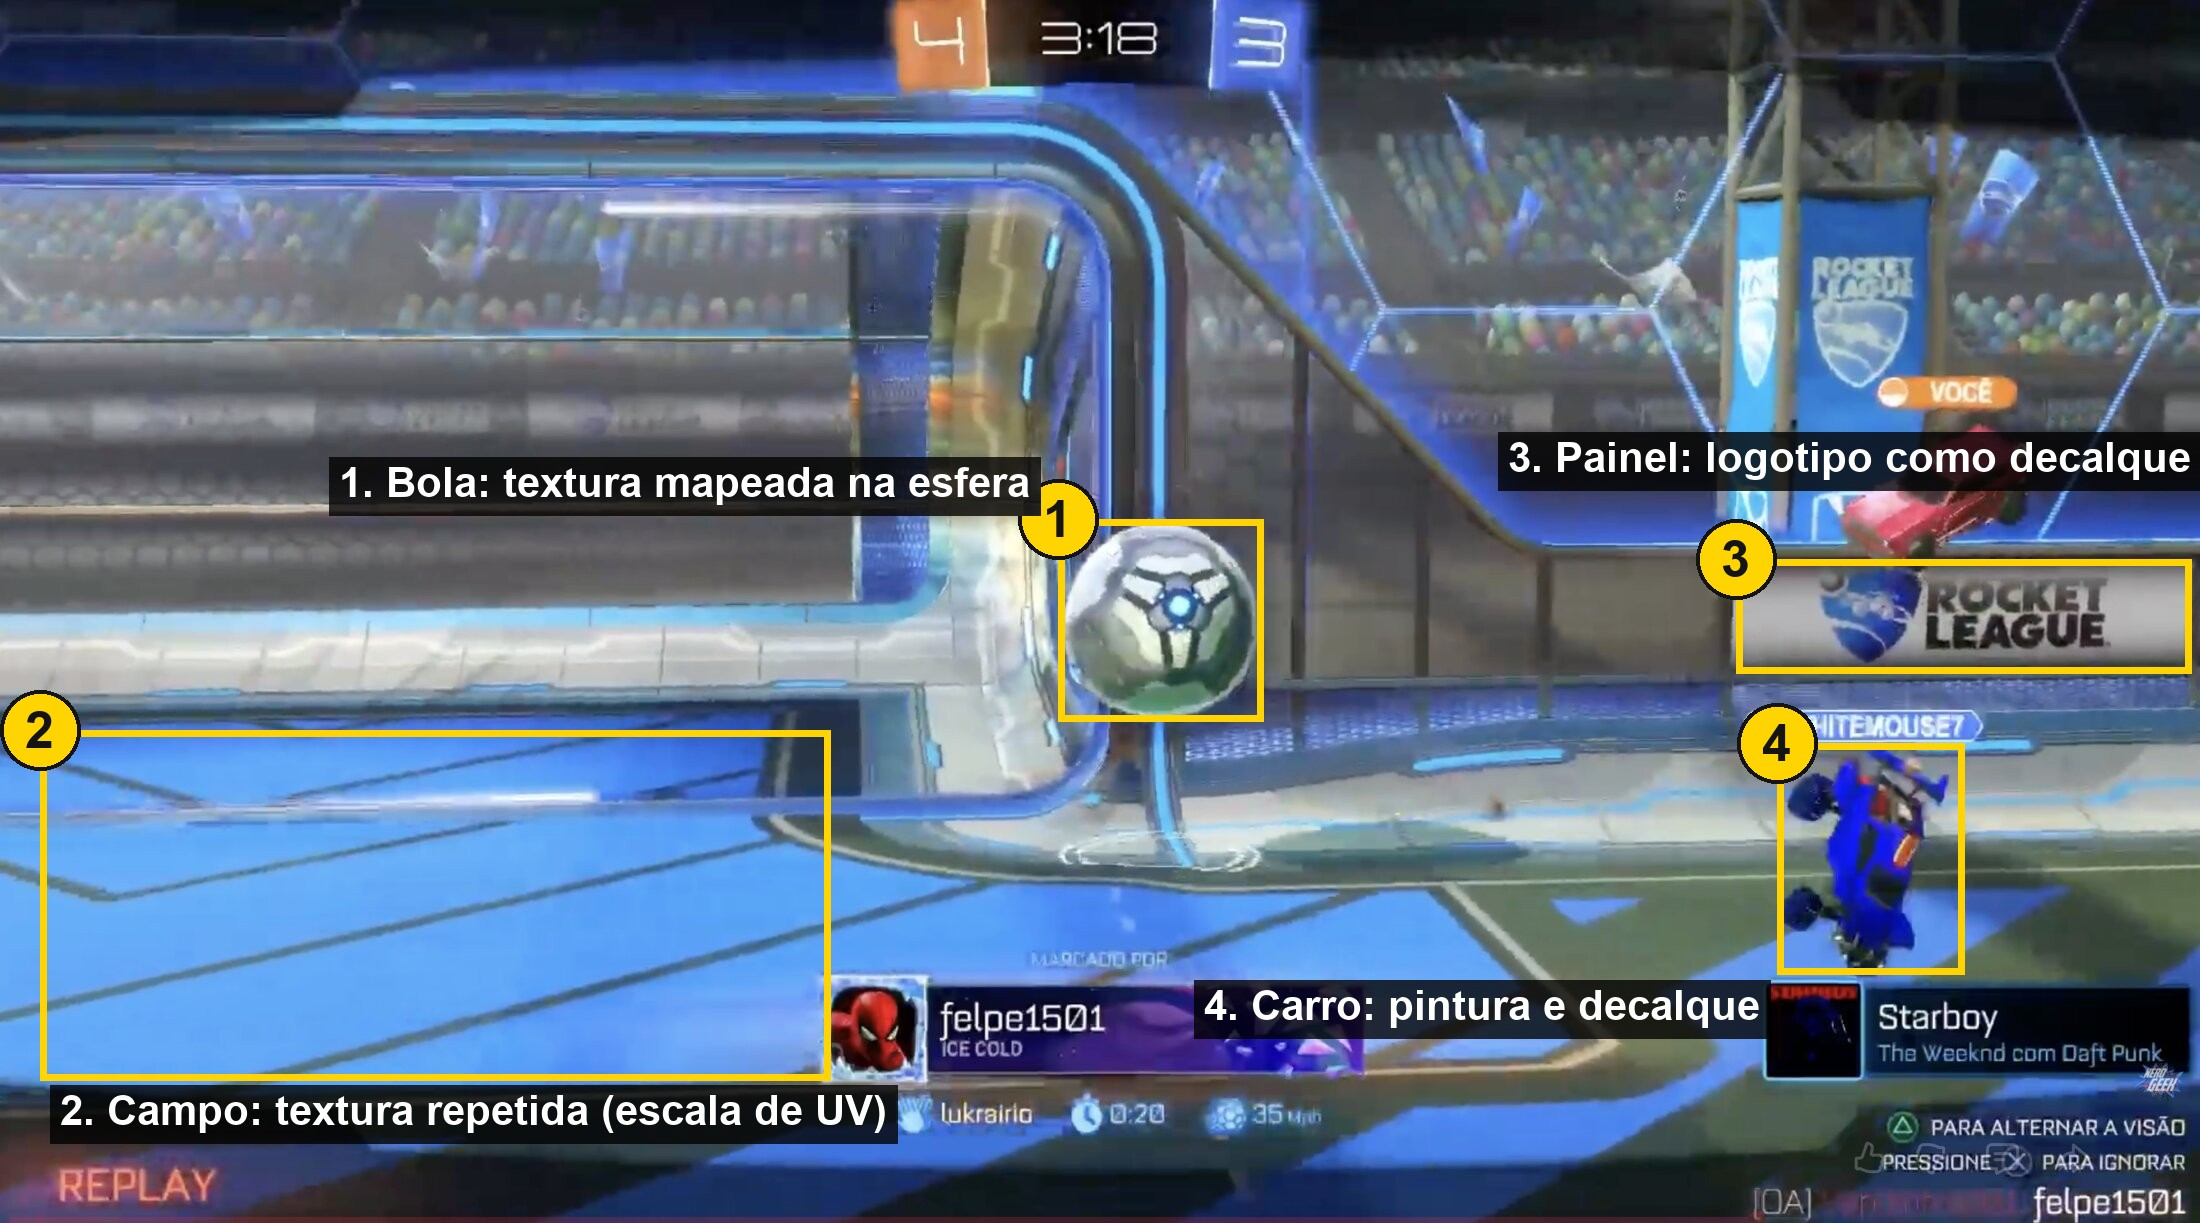
\includegraphics[width=0.92\textwidth]{imagens/marcadas/rl_replay.jpg}
    \caption{Rocket League (PS5), \textit{replay} após um gol. (1)~Bola: textura mapeada na esfera pelo UV. (2)~Campo: o piso e as faixas repetem a mesma textura, ladrilhamento por escala de UV (Eq.~\ref{eq:escala}). (3)~Painel com logotipo: decalque aplicado sobre a região UV do painel. (4)~Carro adversário: pintura sobre o UV do modelo.}
    \label{fig:rl-replay}
\end{figure}

\textbf{Cena da Figura~\ref{fig:rl-garagem}.} Na tela inicial, antes da partida, o jogo exibe o carro do jogador parado no gramado, com a pintura e as rodas escolhidas na garagem.

\begin{figure}[H]
    \centering
    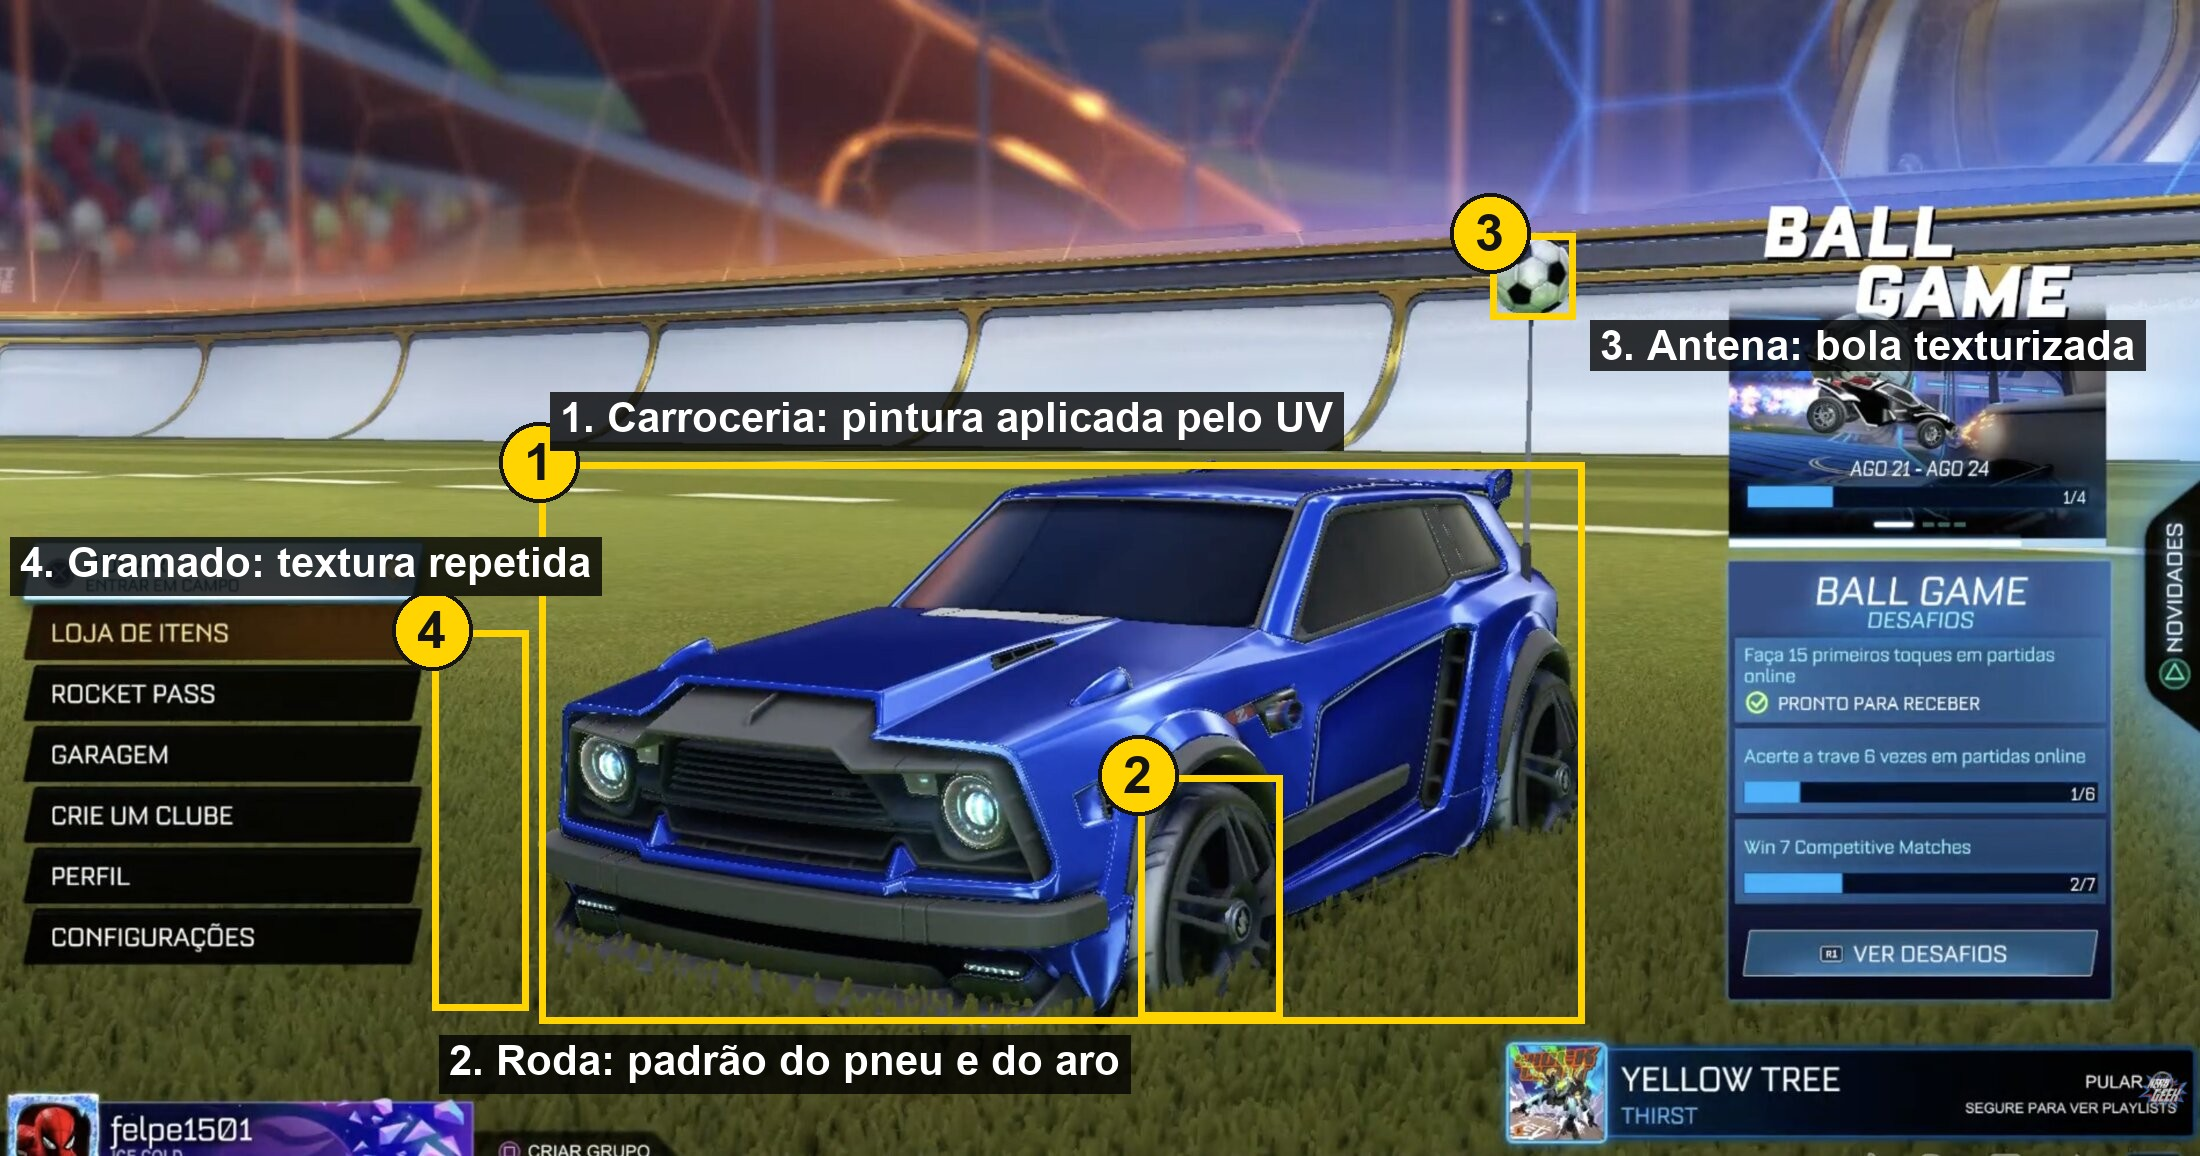
\includegraphics[width=0.92\textwidth]{imagens/marcadas/rl_garagem.jpg}
    \caption{Rocket League (PS5), tela inicial. (1)~Carroceria: a pintura é uma textura sobre o layout UV do carro; os decalques, quando equipados, usam o mesmo layout. (2)~Roda: banda de rodagem e aro gerados proceduralmente no Substance Designer \cite{substance}. (3)~Antena: esfera com textura própria. (4)~Gramado: textura repetida (Eq.~\ref{eq:escala}).}
    \label{fig:rl-garagem}
\end{figure}

\textbf{Vídeo.} Transmissão ao vivo do grupo (PS5): \url{https://www.youtube.com/live/eUX4mfkpFlQ}. Nela aparecem a tela inicial com o carro, os \textit{replays} após os gols e o rastro do \textit{boost} durante as partidas.

\section{Marvel's Spider-Man Remastered}

\begin{table}[H]
\centering
\caption{Análise do Marvel's Spider-Man Remastered.}
\label{tab:ficha-sm}
\small
\begin{tabular}{p{3.0cm}p{11.0cm}}
\toprule
Jogo & \textit{Marvel's Spider-Man Remastered} (Insomniac Games) \\
Plataforma & PlayStation~5, versão nativa, lançada em 12 de novembro de 2020 \cite{spidermanps} \\
Situação analisada & (a) Missão da história em que o Homem-Aranha observa um píer da polícia, em conversa por rádio com a ``Técnica da Torre''; (b) exploração livre no alto de um arranha-céu de Manhattan; (c) menu de pausa, aba \textit{Trajes} \\
Momento & (a) Durante a missão, com o personagem parado na borda do prédio; (b) no instante da notificação de desbloqueio do DLC ``A Cidade que Nunca Dorme''; (c) na escolha do traje \\
Elementos visuais & Fachadas dos prédios; traje do personagem; veículos e piso do píer; água da baía e dos rios \\
Efeito produzido & Janelas repetidas ao longo dos andares; padrão de teia acompanhando a curvatura do corpo; decalques sobre os veículos e o píer; superfície de água com textura de ondas \\
Benefício & As fachadas repetem um módulo de janela, o que permite texturizar uma cidade inteira com poucas imagens. Cada traje é um conjunto de texturas sobre o UV do personagem, o que permite oferecer dezenas de trajes \\
Fonte técnica & Página da Insomniac sobre a versão remasterizada (modelos e materiais melhorados, reflexos com \textit{ray tracing}) \cite{insomniac}. Para a água, a Insomniac não publica a implementação; o uso de UV em deslocamento é justificado pela técnica documentada nos motores \cite{unrealpanner,unitytiling} e demonstrado na implementação do grupo (Seção~\ref{sec:demo-app}) \\
\bottomrule
\end{tabular}
\end{table}

Neste jogo, a técnica aparece com mais clareza no UV tradicional: o padrão de teia dos trajes, os decalques dos veículos e as fachadas com janelas repetidas. A água da baía e dos rios é coberta por uma textura de ondas. Em jogos, superfícies de água desse tipo costumam ser animadas deslocando o UV da textura ao longo do tempo (Equações~\eqref{eq:translacao} e~\eqref{eq:onda}), em vez de deformar a geometria, como no nó \textit{Panner} \cite{unrealpanner}. Como a Insomniac não publica a implementação e uma captura estática não registra movimento, a água é tratada aqui apenas como efeito compatível com a técnica. A demonstração do UV dinâmico em funcionamento é feita na implementação do grupo (Seção~\ref{sec:demo-app}). Os reflexos sobre a água vêm de outra técnica, o \textit{ray tracing} \cite{insomniac}.

\textbf{Cena da Figura~\ref{fig:sm-pier}.} Durante uma missão, o Homem-Aranha está agachado na borda de um prédio, observando um píer com veículos da polícia, enquanto conversa por rádio com a ``Técnica da Torre''. A baía aparece ao fundo.

\begin{figure}[H]
    \centering
    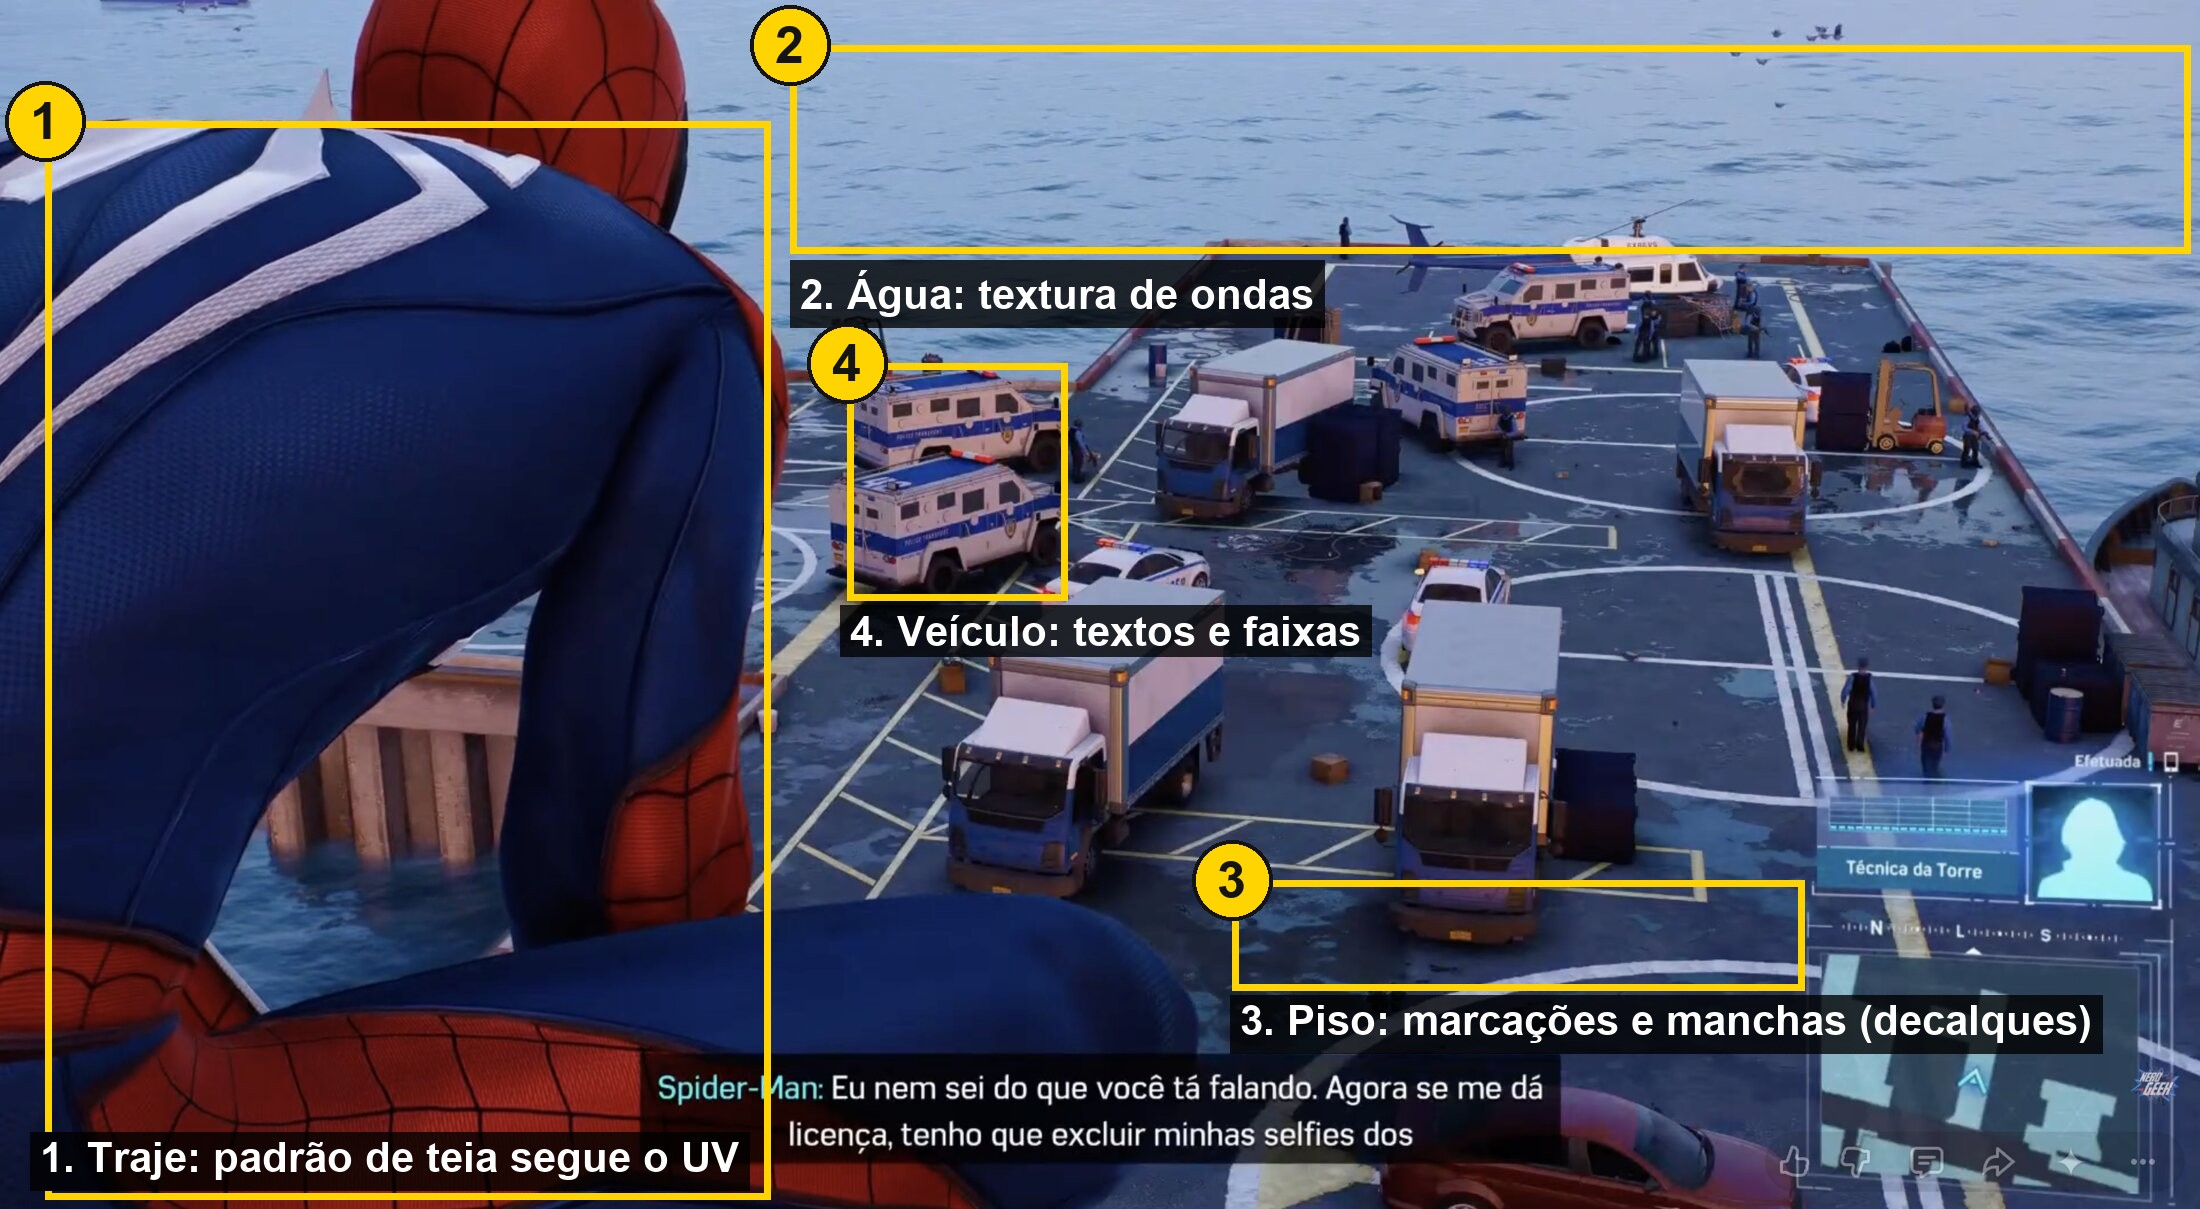
\includegraphics[width=0.92\textwidth]{imagens/marcadas/sm_pier.jpg}
    \caption{Marvel's Spider-Man Remastered (PS5), missão no píer da polícia. (1)~Traje: o padrão de teia e o relevo do tecido seguem o UV do personagem. (2)~Água: superfície coberta por uma textura de ondas; em jogos, esse tipo de superfície costuma ser animado deslocando o UV (Eqs.~\ref{eq:translacao} e~\ref{eq:onda}), o que uma imagem estática não permite confirmar. (3)~Piso do píer: marcações e manchas como decalques sobre uma textura repetida. (4)~Veículos: textos e faixas mapeados pelo UV de cada modelo.}
    \label{fig:sm-pier}
\end{figure}

\textbf{Cena da Figura~\ref{fig:sm-cidade}.} Na exploração livre, o personagem para no alto de um arranha-céu, com Manhattan e o rio à frente, no instante em que o jogo notifica o desbloqueio de um DLC.

\begin{figure}[H]
    \centering
    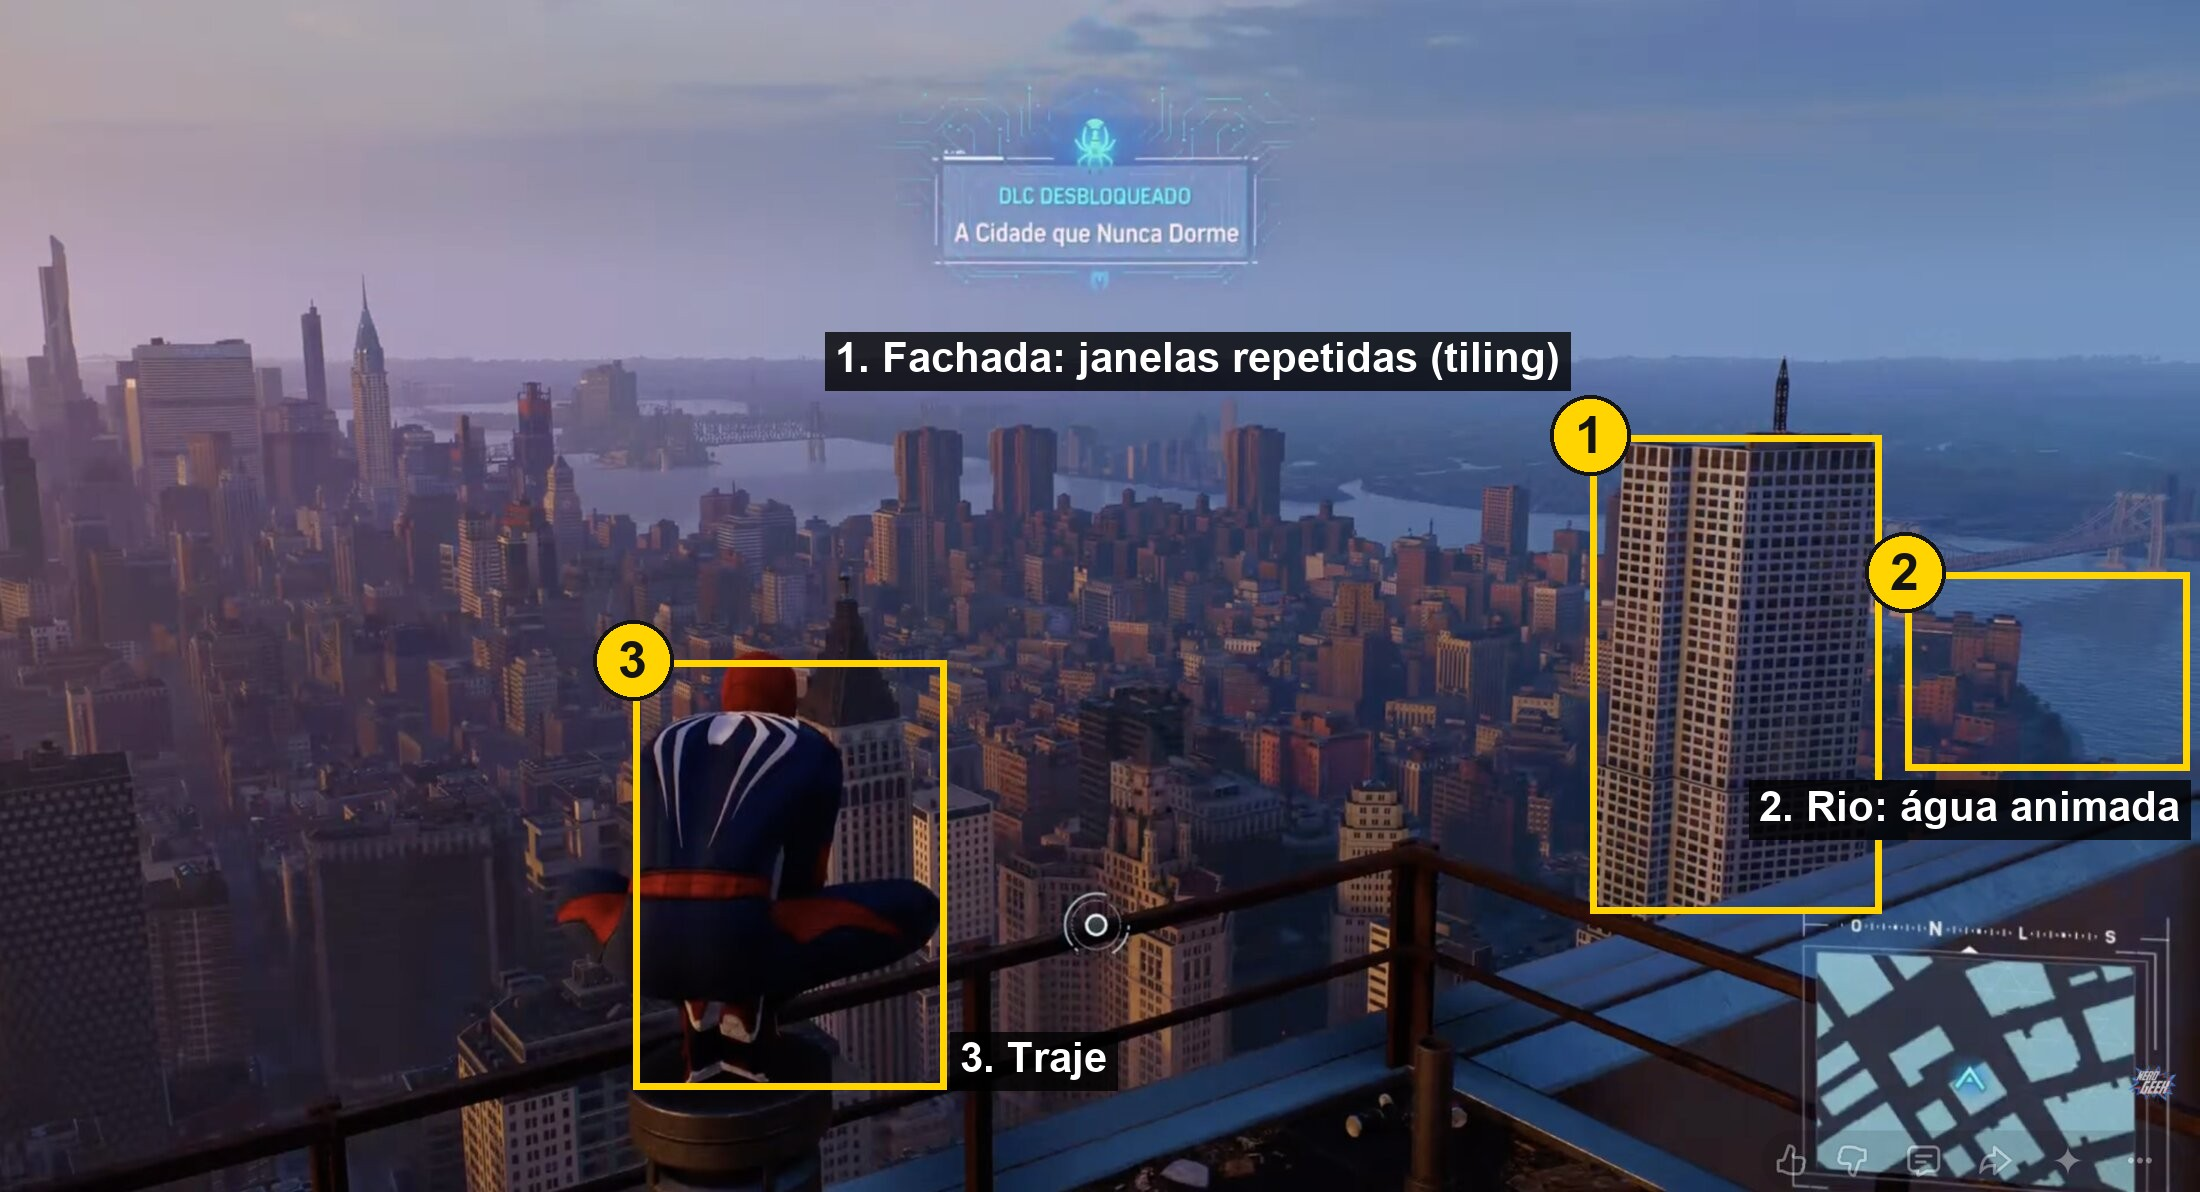
\includegraphics[width=0.92\textwidth]{imagens/marcadas/sm_cidade.jpg}
    \caption{Marvel's Spider-Man Remastered (PS5), exploração livre. (1)~Fachada: o mesmo módulo de janelas se repete ao longo dos andares (Eq.~\ref{eq:escala}). (2)~Rio: superfície de água com textura de ondas, a mesma da Figura~\ref{fig:sm-pier}. (3)~Traje do personagem, mapeado pelo UV.}
    \label{fig:sm-cidade}
\end{figure}

\textbf{Cena da Figura~\ref{fig:sm-trajes}.} No menu de pausa, aba \textit{Trajes}, o jogo exibe o modelo do personagem com o traje selecionado ao lado da lista de trajes desbloqueados.

\begin{figure}[H]
    \centering
    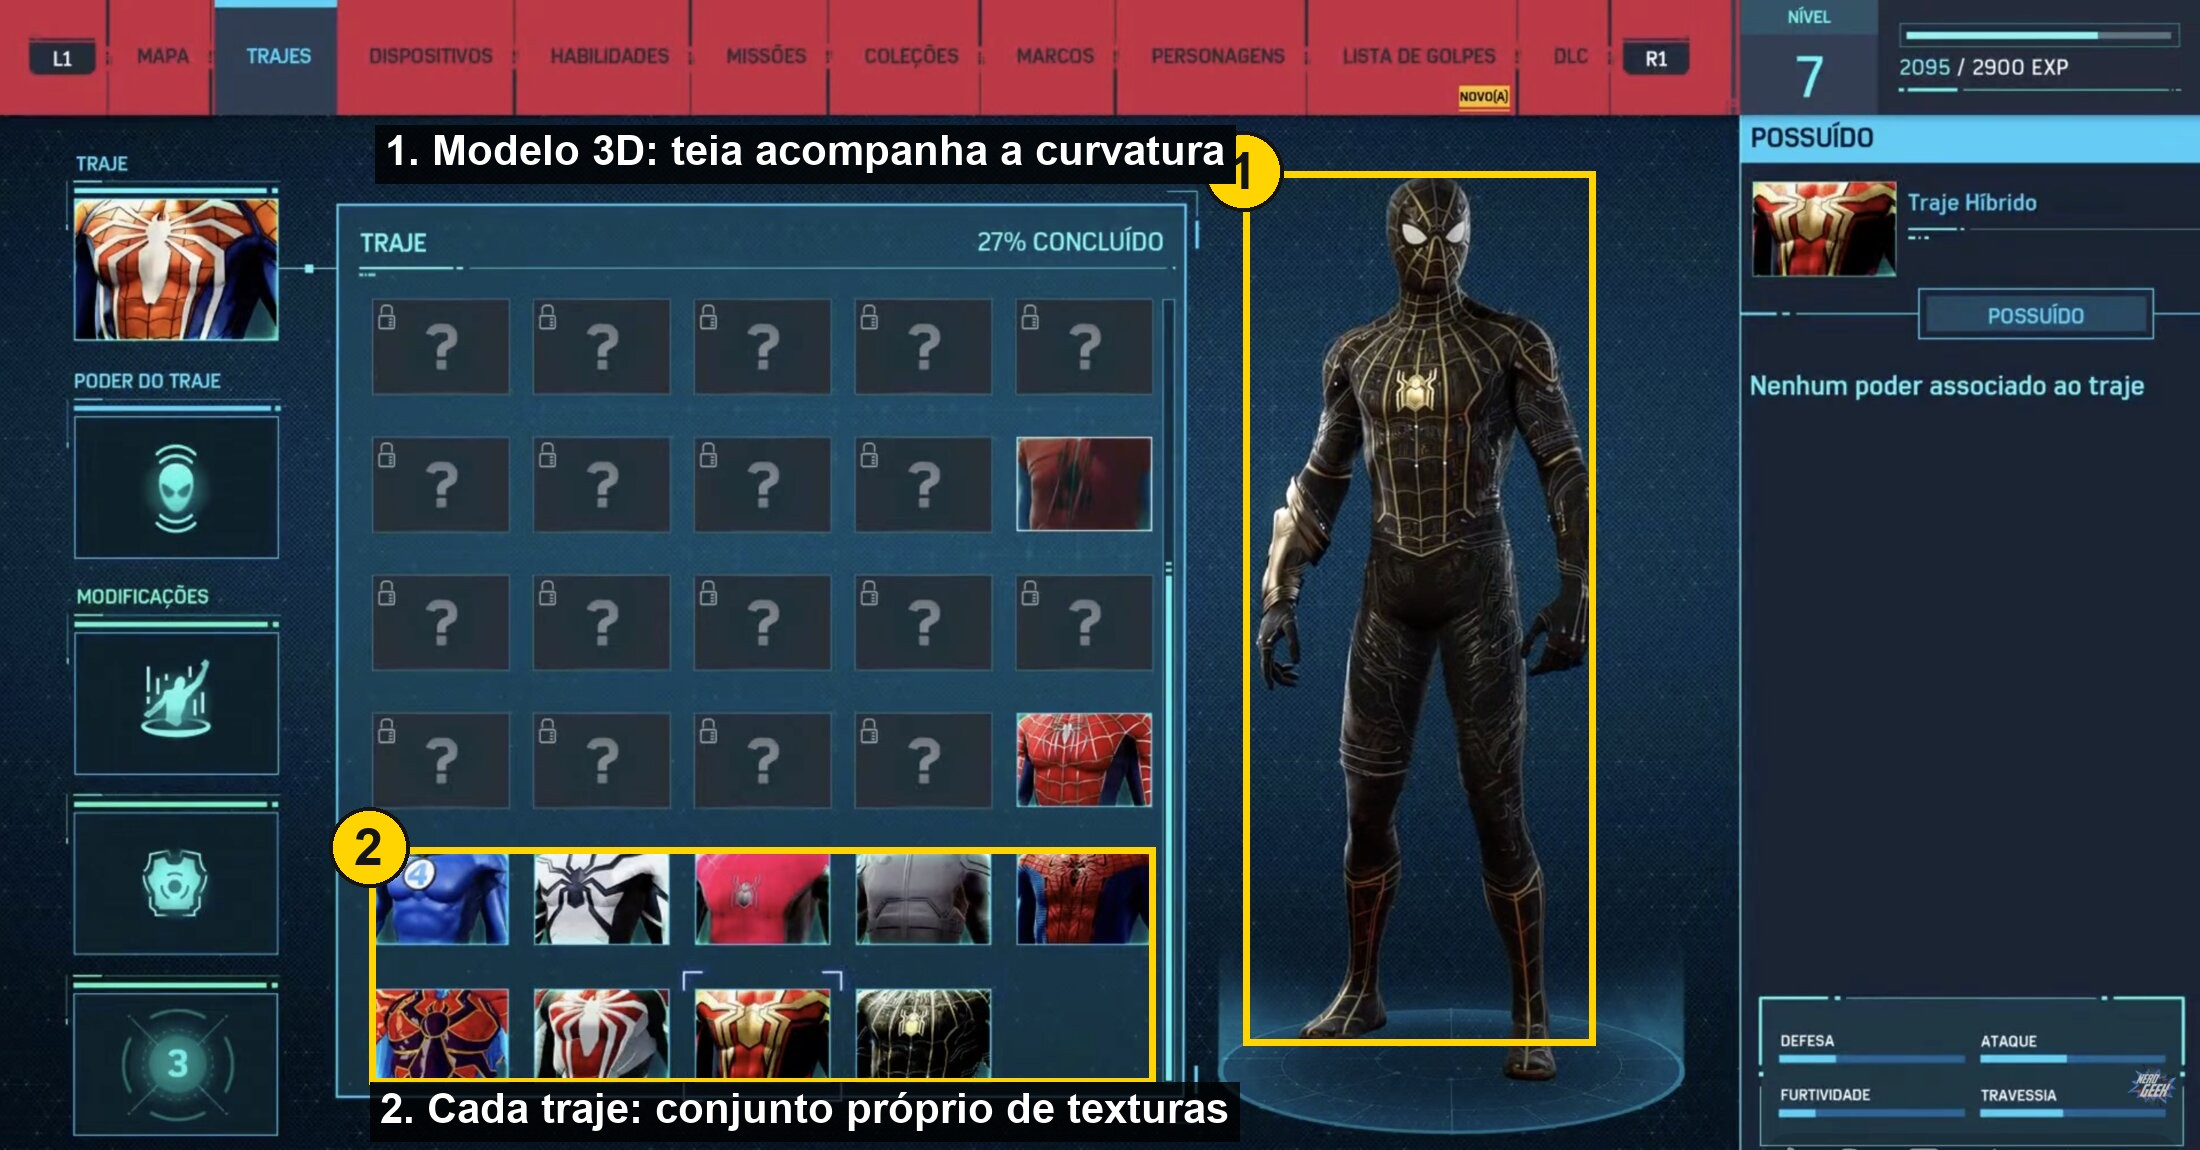
\includegraphics[width=0.92\textwidth]{imagens/marcadas/sm_trajes.jpg}
    \caption{Marvel's Spider-Man Remastered (PS5), menu de trajes. (1)~Modelo do personagem: as linhas da teia acompanham a curvatura do corpo, resultado da parametrização UV. (2)~Lista de trajes: cada traje é um conjunto próprio de texturas.}
    \label{fig:sm-trajes}
\end{figure}

\textbf{Lives completas.} Transmissões ao vivo do grupo (PS5): ``Parte 5'', \url{https://www.youtube.com/live/mhFPk9TQWWA}, e ``Parte 3'', \url{https://www.youtube.com/live/RKo-mqZgxG8}. Nelas aparecem as fachadas durante o balanço pela cidade, a baía e o menu de trajes.

\section{Demonstração na implementação do grupo}
\label{sec:demo-app}

Uma captura estática de um jogo comercial não registra movimento, e o código do jogo não está disponível. Por isso, a Figura~\ref{fig:app-uv-dinamico} demonstra o UV dinâmico na implementação Vulkan do grupo, em que ele pode ser comprovado quadro a quadro. A rotação do modelo foi pausada (tecla Espaço). O primeiro quadro está no modo~1, com a textura original, e os outros três estão no modo~2, com cerca de dois segundos de intervalo. A câmera e a malha não mudam entre os quadros. O olho, marcado com um círculo, começa na cabeça e atravessa o corpo à medida que \(u\) cresce com \(u' = u + 0{,}10\,t\) (Equação~\eqref{eq:translacao}).

\begin{figure}[H]
    \centering
    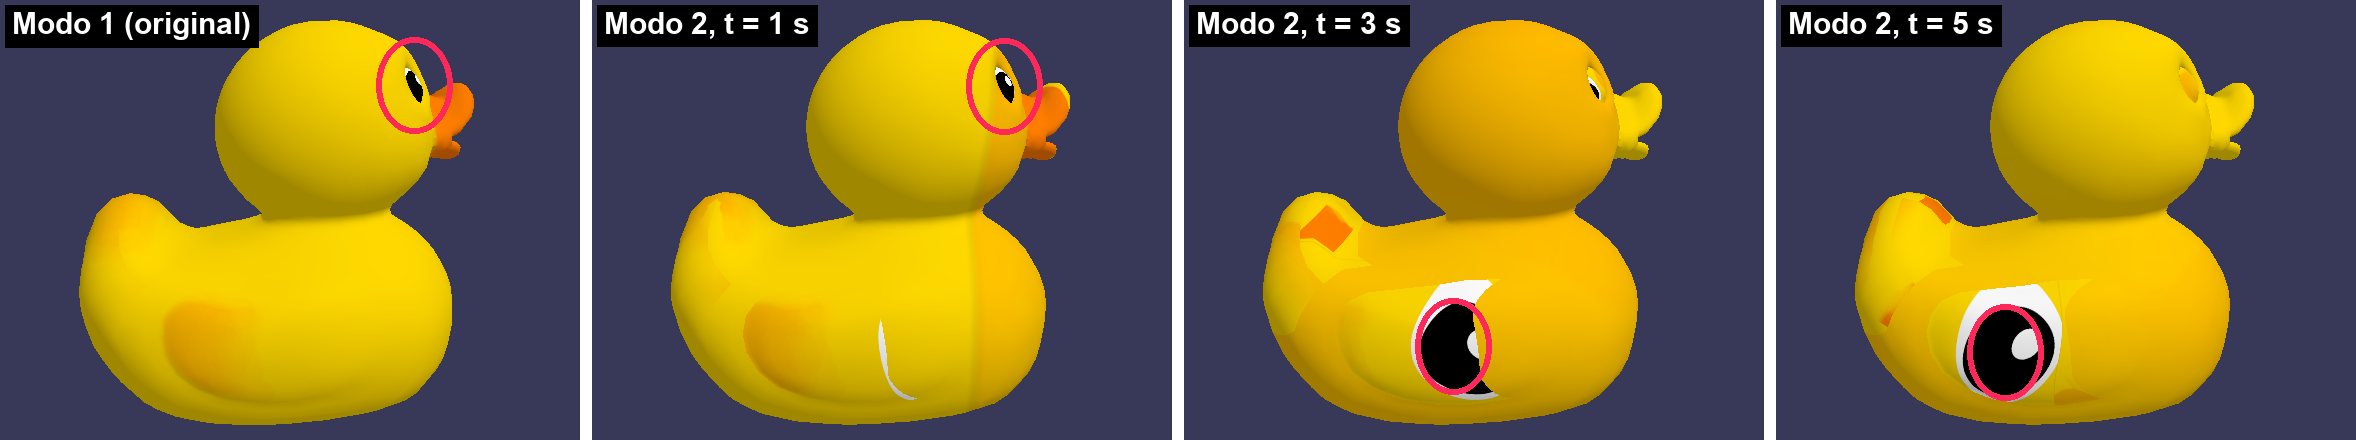
\includegraphics[width=\textwidth]{imagens/marcadas/app_uv_dinamico.png}
    \caption{Captura própria da implementação (Vulkan, \texttt{Duck.glb}): modo~1 e modo~2 em \(t \approx 1\), 3 e 5~s, com a malha parada. O olho (círculo) desliza da cabeça para o corpo porque o UV é deslocado no fragment shader (função \texttt{dynamicUV}).}
    \label{fig:app-uv-dinamico}
\end{figure}

\section{Comparação}

\begin{table}[H]
\centering
\caption{Técnicas observadas e onde aparecem nas capturas.}
\label{tab:marcacoes}
\small
\begin{tabular}{p{3.6cm}p{2.6cm}p{7.6cm}}
\toprule
\textbf{Técnica} & \textbf{Equação} & \textbf{Onde aparece} \\
\midrule
UV tradicional & \eqref{eq:uv}, \eqref{eq:perspectiva} & Fig.~\ref{fig:rl-replay}~(1, 4); Fig.~\ref{fig:rl-garagem}~(1, 3); Fig.~\ref{fig:sm-pier}~(1, 4); Fig.~\ref{fig:sm-cidade}~(3); Fig.~\ref{fig:sm-trajes}~(1, 2) \\
Ladrilhamento por escala & \eqref{eq:escala}, \eqref{eq:repeat} & Fig.~\ref{fig:rl-replay}~(2); Fig.~\ref{fig:rl-garagem}~(4); Fig.~\ref{fig:sm-cidade}~(1) \\
Decalque & \eqref{eq:uv} & Fig.~\ref{fig:rl-replay}~(3); Fig.~\ref{fig:sm-pier}~(3) \\
Procedural (na produção) & --- & Fig.~\ref{fig:rl-garagem}~(2): pneu e aro gerados no Substance Designer \cite{substance} \\
UV dinâmico & \eqref{eq:translacao}, \eqref{eq:onda} & Fig.~\ref{fig:app-uv-dinamico} (comprovado na implementação); Fig.~\ref{fig:sm-pier}~(2) e Fig.~\ref{fig:sm-cidade}~(2) (água, compatível); rastro do \textit{boost} no Rocket League (compatível) \\
\bottomrule
\end{tabular}
\end{table}

Nos dois jogos, o UV tradicional é o que viabiliza a escala do conteúdo: dezenas de carros e trajes personalizáveis e uma cidade inteira texturizada com módulos repetidos. O UV dinâmico é esperado onde o jogo precisa de movimento contínuo e barato: a água no Spider-Man e o rastro do \textit{boost} no Rocket League. Nos dois casos, porém, os estúdios não publicam a implementação, e o rastro do \textit{boost} ainda combina partículas (pequenas imagens que nascem e somem atrás do carro) com o brilho do rastro. Por isso, este trabalho trata esses efeitos como compatíveis com a técnica e demonstra o UV dinâmico em funcionamento na própria implementação (Figura~\ref{fig:app-uv-dinamico}), onde o deslocamento pode ser medido.


\chapter{Resumo das publicações utilizadas}
\label{chap:resumos}

As versões de Heckbert e de Smelik et al.\ incluídas na pasta \texttt{docs/artigos/} são as versões dos autores (\textit{preprints}), cuja paginação difere da revista. As páginas citadas referem-se a essas versões, para que possam ser conferidas nos arquivos entregues. Os mesmos resumos estão em \texttt{docs/resumos/}.

\section{Heckbert (1986)}

\textbf{Título:} \textit{Survey of Texture Mapping}. \textbf{Autor:} Paul S. Heckbert. \textbf{Ano:} 1986 (IEEE Computer Graphics and Applications, v.~6, n.~11) \cite{heckbert1986}.

\textbf{Objetivo.} Organizar o conhecimento sobre texture mapping disponível até meados dos anos 1980, separando o problema em mapeamento geométrico e filtragem \cite[p.~1]{heckbert1986}.

\textbf{Principais conceitos.}
\begin{itemize}
    \item O mapeamento como composição de uma parametrização da superfície com a projeção para a tela \cite[p.~2]{heckbert1986}.
    \item Os parâmetros que podem ser mapeados (cor, normal, especular, transparência, deslocamento) \cite[p.~2]{heckbert1986}.
    \item Os mapeamentos afim, bilinear e projetivo, e a interpolação correta em perspectiva, com uma divisão por pixel \cite[pp.~4--5]{heckbert1986}.
    \item A taxonomia dos filtros (convolução direta, pré-filtragem e séries de Fourier) \cite[p.~7]{heckbert1986}, com uma tabela de custo e memória em que a pirâmide de mipmaps ocupa \(4/3\) da textura e a interpolação trilinear custa 8 acessos por pixel \cite[pp.~9--10]{heckbert1986}.
\end{itemize}

\textbf{Relação com o tema.} É a base do UV mapping: define o espaço \((u,v)\), mostra como ele chega a cada pixel e quanto custa ler a textura corretamente. O UV dinâmico altera justamente a parametrização descrita pelo autor. O artigo é anterior às GPUs programáveis e não trata de UV animado.

\textbf{Informações aproveitadas.} Composição do mapeamento e ordem de varredura (Cap.~\ref{chap:fundamentacao}); interpolação com correção de perspectiva e seleção de mipmap (Cap.~\ref{chap:equacoes}); aliasing, custo da filtragem trilinear e memória dos mipmaps (Caps.~\ref{chap:fundamentacao} e~\ref{chap:vulkan}).

\section{Dong et al. (2020)}

\textbf{Título:} \textit{Survey of Procedural Methods for Two-Dimensional Texture Generation}. \textbf{Autores:} Junyu Dong, Jun Liu, Kang Yao, Mike Chantler, Lin Qi, Hui Yu e Muwei Jian. \textbf{Ano:} 2020 (Sensors, v.~20, n.~4, 1135) \cite{dong2020}.

\textbf{Objetivo.} Revisar e comparar, pela aparência que produzem, os métodos de geração procedural de texturas bidimensionais estáticas. Texturas sólidas, jogos e animação ficam explicitamente fora do escopo \cite[p.~2]{dong2020}.

\textbf{Principais conceitos.}
\begin{itemize}
    \item A definição de textura procedural como imagem criada por um modelo matemático \cite[p.~1]{dong2020}.
    \item A classificação em métodos estruturados (autômatos celulares, reação-difusão, textons, Voronoi, texturas celulares), não estruturados (funções de ruído no domínio da frequência e no espacial, como Gabor e Perlin) e de pós-processamento \cite[pp.~3--4]{dong2020}.
    \item Uma avaliação perceptual de 20 métodos, com 450 amostras e 40 participantes \cite[pp.~19--20]{dong2020}, resumida em uma tabela de aplicações típicas de cada método \cite[p.~22]{dong2020}.
\end{itemize}

\textbf{Relação com o tema.} Fundamenta o lado procedural da técnica: o que é uma textura gerada por função, quando ela é vantajosa (tamanho ilimitado, sem costuras, famílias de variações) e quais são seus problemas (controle de parâmetros, aliasing, dificuldade de reproduzir texturas reais) \cite[pp.~2, 13, 23]{dong2020}.

\textbf{Informações aproveitadas.} Definição e taxonomia do procedural, critérios de quando usar e limitações (Cap.~\ref{chap:fundamentacao}); classificação dos nós procedurais do Blender (Cap.~\ref{chap:aplicacoes}); a ressalva de que o tempo relatado (menos de um segundo por imagem, em computador de mesa) mede a geração de uma imagem inteira, e não a avaliação por fragmento em tempo real \cite[p.~21]{dong2020}.

\section{Smelik et al. (2014)}

\textbf{Título:} \textit{A Survey on Procedural Modelling for Virtual Worlds}. \textbf{Autores:} Ruben M. Smelik, Tim Tutenel, Rafael Bidarra e Bedrich Benes. \textbf{Ano:} 2014 (Computer Graphics Forum, v.~33, n.~6) \cite{smelik2014}.

\textbf{Objetivo.} Revisar os métodos de modelagem procedural para mundos virtuais e entender por que eles ainda são pouco adotados por profissionais criativos \cite[p.~1]{smelik2014}.

\textbf{Principais conceitos.}
\begin{itemize}
    \item A amplificação de dados: poucos parâmetros geram grande variedade de conteúdo, inclusive sob demanda na GPU \cite[p.~1]{smelik2014}.
    \item A organização dos métodos por tipo de conteúdo (terreno, vegetação, água, estradas, cidades, edifícios, interiores) e a avaliação de cada um por facilidade de uso, controle e família de técnica \cite[p.~2]{smelik2014}.
    \item Uma seção sobre sistemas comerciais (Terragen, SpeedTree, CityEngine, Houdini) \cite[pp.~10--12]{smelik2014}.
    \item Os dois obstáculos à adoção: a falta de controle intuitivo e a falta de integração entre métodos \cite[pp.~12--15]{smelik2014}.
\end{itemize}

\textbf{Relação com o tema.} Mostra o procedural em escala de mundo e o problema de controle que também afeta as texturas procedurais. O levantamento exclui a geração de texturas \cite[p.~2]{smelik2014}, por isso é usado para o contexto de produção e para os produtos reais, e não para a texturização em si.

\textbf{Informações aproveitadas.} Amplificação de dados e custo da produção manual (quando usar), baixa controlabilidade e desempenho interativo (limitações e custo) (Cap.~\ref{chap:fundamentacao}); SpeedTree, CityEngine, Houdini e Substance Designer como produtos reais (Cap.~\ref{chap:aplicacoes}).

\section{Relação entre as publicações}

As três publicações cobrem camadas diferentes do problema. Heckbert trata de como uma coordenada \((u,v)\) chega a um pixel e quanto custa ler a textura. Dong et al.\ tratam do conteúdo procedural da textura em si. Smelik et al.\ tratam do procedural em escala de mundo e do problema de controle que limita seu uso. Nenhuma delas trata diretamente do UV dinâmico em tempo real. Esse ponto é coberto pela implementação do grupo e pelas fontes técnicas dos motores e estúdios (Capítulos~\ref{chap:vulkan}, \ref{chap:aplicacoes} e~\ref{chap:jogos}).


\chapter{Conclusão}
\label{chap:conclusao}

O UV mapping associa cada ponto de uma superfície 3D a um ponto de uma textura 2D. Seguindo Heckbert \cite[p.~2]{heckbert1986}, o processo foi tratado como a composição de uma parametrização da superfície com a projeção para a tela. O UV dinâmico altera essa parametrização a cada quadro sem tocar na malha, e o mapeamento procedural substitui a imagem por uma função matemática \cite[p.~1]{dong2020}.

As três abordagens resolvem problemas diferentes. O UV tradicional é a escolha para detalhes únicos e posicionais, como rostos, logotipos e decalques. O UV dinâmico é a escolha para movimento repetitivo (água, lava, esteiras, campos de energia), com o custo de uma amostragem e poucas operações por fragmento. O procedural é a escolha para grandes áreas sem repetição e para famílias de variações \cite[p.~2]{dong2020}. Em troca, ele exige mais cálculo por fragmento, não tem mipmaps que o protejam do aliasing e é difícil de controlar. Dong et al.\ descrevem o ajuste de parâmetros como um processo demorado \cite[p.~23]{dong2020}, e Smelik et al.\ apontam a baixa controlabilidade como o principal motivo de os métodos procedurais ainda não substituírem a modelagem manual \cite[p.~1]{smelik2014}.

A análise das equações mostrou que a pergunta mais importante para o desempenho é onde cada cálculo é executado. Transformações lineares podem ir para a CPU ou para o vertex shader. Deformações não lineares e funções procedurais precisam ficar no fragment shader, que executa centenas de vezes mais que o vertex shader no modelo usado. No Vulkan, a técnica depende de um sampler com endereçamento \texttt{REPEAT}, de um descriptor set que exponha a textura e os parâmetros, e de um mecanismo para enviar o tempo a cada quadro. A implementação usa um Uniform Buffer porque os command buffers são pré-gravados; push constants seriam a alternativa natural se fossem regravados por quadro.

Os produtos analisados mostram as duas formas de uso na indústria. Nos motores de jogo, o UV dinâmico é um recurso de material executado em tempo real, como o \textit{Panner} da Unreal e o \textit{Tiling And Offset} da Unity. Nas ferramentas de autoria, como Substance Designer, SpeedTree e CityEngine, o procedural é usado durante a produção. No Rocket League, as texturas das arenas e das rodas são criadas com o Substance Designer durante a produção, e o jogo as aplica como texturas comuns sobre o UV de cada modelo \cite{substance}. No Marvel's Spider-Man Remastered, a técnica aparece nos trajes, nos decalques e nas fachadas repetidas, e a água da baía é um caso compatível com UV dinâmico. Como os estúdios não publicam a implementação desses efeitos, o UV dinâmico em funcionamento foi demonstrado na implementação do grupo, em que o deslocamento da textura pode ser medido quadro a quadro.

A implementação entregue tem limitações conhecidas, discutidas ao longo do texto: a textura não tem mipmaps, o tempo não é mantido periódico, a translação de UV ainda é feita por pixel e a grade procedural não tem antialiasing analítico. Esses pontos são o caminho natural para uma próxima versão, junto com a divisão dos parâmetros entre Uniform Buffer e push constants.



\printbibliography[heading=bibintoc,title={Referências}]

\appendix

\chapter{Checklist das entregas}

\textbf{Entrega 1 -- Revisão bibliográfica}
\begin{itemize}
    \item[$\boxtimes$] Definição, funcionamento, problema resolvido, vantagens, limitações, custo e quando usar (Capítulo~\ref{chap:fundamentacao}).
    \item[$\boxtimes$] Três publicações científicas citadas ao longo do texto, com um resumo de cada (Capítulo~\ref{chap:resumos} e \texttt{resumos/}).
    \item[$\boxtimes$] Equações com variáveis, finalidade, momento de uso e relação com a renderização (Capítulo~\ref{chap:equacoes}).
    \item[$\boxtimes$] Relação com o Vulkan: shaders, estágios, buffers, texturas, attachments, fluxo de dados e otimizações (Capítulo~\ref{chap:vulkan}).
    \item[$\boxtimes$] Sete aplicações reais, com onde a técnica é usada e o benefício (Capítulo~\ref{chap:aplicacoes}).
    \item[$\boxtimes$] Dois jogos, com plataforma, situação, momento, elemento, efeito, benefício e fonte técnica (Capítulo~\ref{chap:jogos}).
    \item[$\boxtimes$] Capturas próprias marcadas, com legenda e texto da cena (Capítulo~\ref{chap:jogos}).
    \item[$\boxtimes$] Links das lives de gameplay do grupo no PDF e em \texttt{videos.txt}; demonstração do UV dinâmico em funcionamento na implementação (Figura~\ref{fig:app-uv-dinamico}).
\end{itemize}

\textbf{Entrega 2 -- Arquitetura do pipeline Vulkan}
\begin{itemize}
    \item[$\boxtimes$] Diagrama com legenda de cores e setas, e arquivo-fonte \texttt{diagrama/pipeline\_vulkan.dot} (Figura~\ref{fig:pipeline-vulkan}).
    \item[$\boxtimes$] Fluxo de dados, com entradas e saídas de cada estágio (Tabela~\ref{tab:estagios}).
    \item[$\boxtimes$] Render Pass, Subpass e attachments; descriptor sets e bindings; layout e finalidade dos buffers (Capítulo~\ref{chap:vulkan}).
    \item[$\boxtimes$] Barreiras de memória e dependência do subpass com todos os campos, transições de layout e dependências entre CPU e GPU (Tabelas~\ref{tab:image-barrier} e~\ref{tab:subpass-dep}).
    \item[$\boxtimes$] Justificativa das decisões arquiteturais (Capítulo~\ref{chap:vulkan}).
\end{itemize}

\textbf{Entrega 3 -- Shaders}
\begin{itemize}
    \item[$\boxtimes$] Pseudocódigo original em \texttt{pseudocodigo/uv\_mapping.vert} e \texttt{.frag}; shaders finais comentados no Capítulo~\ref{chap:shaders}.
    \item[$\boxtimes$] Objetivo, fluxo, entradas e saídas, equações, condições, amostragem, tratamento de limites e resultado esperado (Capítulo~\ref{chap:shaders}).
\end{itemize}

\textbf{Entrega 4 -- Código}
\begin{itemize}
    \item[$\boxtimes$] Aplicação Vulkan em C++ com shaders em SPIR-V, instruções de compilação e evidências de execução (\texttt{código/} e seu \texttt{README.md}).
\end{itemize}

\end{document}
